% =====================================================================
%  Construção de Banco de Dados — UFRJ
%  Tarefa: Dispositivos de Armazenamento Físico para SBD
% =====================================================================
\documentclass[11pt,a4paper]{article}

\usepackage[T1]{fontenc}
\usepackage[utf8]{inputenc}
\usepackage[portuges]{babel}
\usepackage{lmodern}
\usepackage{amsmath,amssymb}
\usepackage[a4paper,left=2.6cm,right=2.4cm,top=2.6cm,bottom=2.4cm]{geometry}
\usepackage{booktabs,longtable,array,tabularx,multirow,makecell}
\usepackage{graphicx,xcolor,microtype,enumitem,ragged2e,float}
\usepackage{pdflscape}
\usepackage{caption}
\usepackage{fancyhdr}
\usepackage{titlesec}
\usepackage[hidelinks]{hyperref}

\definecolor{azul}{HTML}{2A78D6}
\definecolor{laranja}{HTML}{EB6834}
\definecolor{tinta}{HTML}{0B0B0B}
\definecolor{tinta2}{HTML}{52514E}
\definecolor{linha}{HTML}{E3E2DE}
\definecolor{fundo}{HTML}{F6F6F4}

\hypersetup{colorlinks=true,linkcolor=azul,urlcolor=azul,citecolor=azul}

\captionsetup{font=small,labelfont={bf,color=tinta},textfont={color=tinta2},
              justification=justified,singlelinecheck=false,skip=6pt}

\titleformat{\section}{\Large\bfseries\color{tinta}}{\thesection}{0.6em}{}
\titleformat{\subsection}{\large\bfseries\color{tinta}}{\thesubsection}{0.6em}{}
\titleformat{\subsubsection}{\normalsize\bfseries\color{tinta2}}{\thesubsubsection}{0.6em}{}
\titlespacing*{\section}{0pt}{18pt}{8pt}
\titlespacing*{\subsection}{0pt}{14pt}{6pt}

\pagestyle{fancy}\fancyhf{}
\fancyhead[L]{\footnotesize\color{tinta2}Armazenamento Físico para SBD — CBD/UFRJ}
\fancyhead[R]{\footnotesize\color{tinta2}\thepage}
\renewcommand{\headrulewidth}{0.4pt}
\renewcommand{\headrule}{\color{linha}\hrule height 0.4pt}

\setlist{itemsep=2pt,parsep=0pt,topsep=4pt}
\setlength{\parskip}{4pt}
\setlength{\parindent}{0pt}
\renewcommand{\arraystretch}{1.18}

% caixa de destaque
\newcommand{\destaque}[2]{%
  \begin{center}\begin{minipage}{0.96\textwidth}
  \colorbox{fundo}{\begin{minipage}{\dimexpr\linewidth-2\fboxsep}
  \vspace{3pt}\textbf{\color{azul}#1}\\[2pt]\small #2\vspace{4pt}
  \end{minipage}}\end{minipage}\end{center}}

\newcommand{\correcao}[2]{%
  \begin{center}\begin{minipage}{0.96\textwidth}
  \colorbox{fundo}{\begin{minipage}{\dimexpr\linewidth-2\fboxsep}
  \vspace{3pt}\textbf{\color{laranja}#1}\\[2pt]\small #2\vspace{4pt}
  \end{minipage}}\end{minipage}\end{center}}

\begin{document}

% =====================================================================
% FOLHA DE ROSTO
% =====================================================================
\thispagestyle{empty}
\begin{center}
\vspace*{0.6cm}
{\large\scshape Universidade Federal do Rio de Janeiro}\\[2pt]
{\normalsize Instituto de Matemática --- Departamento de Ciência da Computação}\\[2pt]
{\normalsize Disciplina: \textbf{Construção de Banco de Dados}}\\[2pt]
{\normalsize Professor: Milton Ramirez}\\[1.6cm]

{\color{linha}\rule{\textwidth}{1.2pt}}\\[0.7cm]
{\LARGE\bfseries Dispositivos de Armazenamento Físico\\[6pt] para Sistemas de Banco de Dados}\\[0.5cm]
{\large Interfaces de Conexão e Parâmetros para o\\ Gerente de Armazenamento do SBD}\\[0.5cm]
{\normalsize\itshape Atualização da Tabela 16.1 (Elmasri \& Navathe, 7\textsuperscript{a} ed.)\\ dados consultados em 05 de setembro de 2026}\\[0.6cm]
{\color{linha}\rule{\textwidth}{1.2pt}}\\[1.4cm]

{\large\bfseries Integrantes do Grupo}\\[0.5cm]
\begin{minipage}{0.85\textwidth}\centering
\begin{tabular}{@{}p{9.2cm}p{3.4cm}@{}}
\toprule
\textbf{Nome completo} & \textbf{DRE} \\
\midrule
{}[NOME COMPLETO DO INTEGRANTE 1] & [DRE] \\
{}[NOME COMPLETO DO INTEGRANTE 2] & [DRE] \\
{}[NOME COMPLETO DO INTEGRANTE 3] & [DRE] \\
{}[NOME COMPLETO DO INTEGRANTE 4] & [DRE] \\
{}[NOME COMPLETO DO INTEGRANTE 5] & [DRE] \\
\bottomrule
\end{tabular}
\end{minipage}

\vfill
{\normalsize Rio de Janeiro --- Setembro de 2026}
\end{center}
\newpage

% =====================================================================
\thispagestyle{empty}
\section*{Resumo}
\addcontentsline{toc}{section}{Resumo}

Este trabalho realiza um estudo sobre dispositivos de armazenamento físico para Sistemas
de Banco de Dados (SBD), suas interfaces de conexão e os parâmetros relevantes para o
\emph{Gerente de Armazenamento} do SBD. Partindo do Capítulo~16 de Elmasri \& Navathe
(7\textsuperscript{a} ed.) e do Capítulo~12 de Silberschatz, Korth \& Sudarshan
(7\textsuperscript{a} ed.), o estudo entrega três produtos técnicos:
\textbf{(i)} uma revisão dos fundamentos da hierarquia de memória, da mecânica do disco
magnético, da física da memória \emph{flash} e do estado atual da memória de classe de
armazenamento; \textbf{(ii)} a \textbf{atualização integral da Tabela~16.1} substituindo
cada categoria genérica por produtos comercialmente disponíveis em 2026, com capacidade,
tempo de acesso, largura de banda \emph{segregada em leitura e escrita}, faixa de preço
corrente e uma nova coluna de \textbf{preço por kilobyte}; e \textbf{(iii)} uma tabela
comparativa de cinquenta e seis variantes de interface de conexão (USB, SCSI, SATA, eSATA,
SATA Express, SAS, PCIe/NVMe e seus fatores de forma M.2, U.2, U.3 e EDSFF, NVMe-oF, iSCSI,
FireWire, HBA, Fibre Channel, FCIP, FCoE e InfiniBand), analisando serialidade, codificação
de linha, latência, taxa útil, distância e portabilidade.

Os achados principais contrariam três expectativas correntes na literatura didática.
Primeiro, a memória persistente byte-endereçável \textbf{desapareceu do mercado}: o
Intel Optane foi descontinuado e o vazio de três ordens de grandeza entre DRAM
($\approx$70\,ns) e SSD NVMe ($\approx$50\,\textmu s) só é parcialmente preenchido por
módulos CXL, que medem 214--271\,ns --- duas a duas vezes e meia a latência da DRAM local, e
ainda a três ordens de grandeza do NVMe. Segundo, SSD e HDD \textbf{divergiram em vez de convergir} em custo por
terabyte, com razão de 16$\times$ no 2\textsuperscript{o} trimestre de 2026 e
18,6$\times$ na observação parcial de 05/09/2026. Terceiro, o desempenho de um
SBD moderno é governado por \textbf{latência e profundidade de fila}, não por largura de
banda --- o que explica por que o SATA morreu tecnicamente em 6\,Gb/s sem que ninguém se
importasse, e por que o NVMe venceu.

O documento inclui uma seção obrigatória de \textbf{Post-Mortem} com o log dos prompts-chave
utilizados, a demonstração de autoria dos participantes e o registro auditável dos erros
gerados pelo assistente de IA e das respectivas correções feitas pelo grupo --- entre elas
a correção de uma afirmação factualmente incorreta presente no próprio enunciado da tarefa
(``SATA também é conhecida como NL-SAS'').

\vspace{0.8cm}
\textbf{Palavras-chave:} hierarquia de memória; SSD NVMe; HAMR; LTO-10; CXL; Fibre Channel;
InfiniBand; gerente de armazenamento; latência de \emph{commit}.

\newpage
\thispagestyle{empty}
\tableofcontents
\newpage
\setcounter{page}{1}

% =====================================================================
\section{Introdução}

\subsection{Motivação}

Um Sistema de Gerência de Banco de Dados (SGBD) é, em última análise, uma máquina de
transformar acessos a disco em respostas a consultas. Todas as estruturas centrais da
disciplina --- organização de arquivos, \emph{hashing}, índices B\textsuperscript{+}-tree,
processamento e otimização de consultas, controle de concorrência e recuperação ---
existem porque o meio de armazenamento persistente é ordens de grandeza mais lento que a
memória principal. O modelo de custo do otimizador de consultas conta \emph{blocos lidos};
o gerente de \emph{buffer} existe para evitar releituras; o \emph{log de escrita
antecipada} (WAL) existe porque a escrita no meio persistente é cara e precisa ser
sequencial.

Ocorre que a razão entre essas velocidades --- o parâmetro que justifica toda a
arquitetura --- \textbf{mudou de valor por várias ordens de grandeza} desde que os livros
textos da disciplina foram escritos. A Tabela~16.1 de Elmasri \& Navathe traz preços de
2014; o Capítulo~12 de Silberschatz traz números de 2018. Em 2026, o disco magnético
deixou de ser ``o'' meio secundário de bancos de dados de produção, a memória persistente
que prometia mudar tudo foi descontinuada, e apareceram interfaces que tornaram o
barramento irrelevante como gargalo. Este trabalho mede essa distância.

\subsection{Objetivos}

\begin{enumerate}[label=\textbf{O\arabic*.}]
\item Revisar os fundamentos dos sistemas de armazenamento físico para SBD, articulando o
      tratamento de Elmasri \& Navathe (Cap.~16), Silberschatz \emph{et al.} (Cap.~12) e
      Garcia-Molina, Ullman \& Widom (Cap.~13).
\item Atualizar integralmente a Tabela~16.1, substituindo cada tipo genérico de
      \emph{storage} por exemplos comercialmente disponíveis em 2026, com faixas de preço
      correntes, largura de banda segregada em leitura e escrita, e uma coluna adicional
      de \textbf{preço por kilobyte}.
\item Elaborar uma tabela comparativa das interfaces de conexão entre o dispositivo físico
      e o sistema computacional, contemplando serialidade, latência, taxa máxima de
      transferência, portabilidade e distância máxima.
\item Traduzir esses números em \textbf{parâmetros acionáveis para o Gerente de
      Armazenamento do SBD}: tamanho de bloco, política de \emph{buffer}, latência de
      \emph{commit}, modelo de custo do otimizador e estratégia de \emph{tiering}.
\item Registrar, em Post-Mortem auditável, o uso de assistentes de IA generativa: o que foi
      pedido, o que a IA errou, quem detectou e como foi corrigido.
\end{enumerate}

\subsection{Metodologia e critérios de seleção}

A pesquisa combinou três fontes. \textbf{(a)~Fontes textuais primárias:} os capítulos dos
livros-texto indicados no enunciado, lidos integralmente para extrair os parâmetros
originais e a taxonomia. Os três cumprem papéis distintos e complementares: Elmasri \&
Navathe detalham as arquiteturas modernas (SAN, NAS, iSCSI, \emph{tiering}, armazenamento
por objetos) e fornecem a Tabela~16.1 que este trabalho atualiza; Silberschatz \emph{et al.}
detalham a física do \emph{flash}, a \emph{Flash Translation Layer} e as métricas de disco;
e Garcia-Molina, Ullman \& Widom (Cap.~13) fornecem a formalização do \textbf{\emph{I/O
model of computation}}, que é o elo entre os parâmetros físicos deste estudo e o modelo de
custo do otimizador --- e que a Seção~5.5 usa para mostrar por que esse modelo envelheceu. \textbf{(b)~Especificações normativas:} documentos publicados
pelos organismos que definem cada interface --- USB-IF, SATA-IO, INCITS/T10 (SCSI e SAS),
INCITS/T11 (Fibre Channel), NVM Express Inc., PCI-SIG, IEEE, IETF (RFC 7143), IBTA
(InfiniBand), CXL Consortium, SNIA e o LTO Program. \textbf{(c)~Documentação de
fabricante:} \emph{datasheets} e manuais de produto, complementados por preços de referência
consultados em 05 de setembro de 2026.

Para a escolha dos dispositivos da Tabela~16.1 atualizada, o grupo adotou três critérios,
nesta ordem de precedência:

\begin{enumerate}[label=\textbf{C\arabic*.}]
\item \textbf{Disponibilidade das quatro informações exigidas pelo enunciado} (capacidade,
      tempo de acesso, largura de banda e preço). Produtos tecnicamente mais interessantes
      foram preteridos quando o fabricante não publica um dos quatro valores.
\item \textbf{Representatividade de mercado}: preferência por produtos em produção corrente
      e com preço de varejo público verificável, e não por protótipos ou peças de
      demonstração.
\item \textbf{Rastreabilidade}: cada célula tem origem declarada --- \emph{datasheet} do
      fabricante, medição de terceiro, derivação aritmética explícita ou estimativa.
\end{enumerate}

\destaque{Convenção de unidades adotada}{%
Este documento distingue rigorosamente \textbf{bit} (b) de \textbf{byte} (B):
1\,GB/s $=$ 8\,Gb/s. Para \textbf{dispositivos de armazenamento} adota-se a convenção
decimal da indústria (1\,KB $=$ 10\textsuperscript{3}\,B, 1\,TB $=$
10\textsuperscript{12}\,B); para \textbf{memórias} (SRAM, DRAM) adota-se a convenção
binária JEDEC (1\,KB $=$ 2\textsuperscript{10}\,B). A coluna ``preço por KB'' foi
calculada dentro da convenção própria de cada categoria, e o resultado é apresentado em
notação científica porque a faixa cobre seis ordens de grandeza.}

\subsection{Estrutura do documento}

A Seção~2 revisa os fundamentos. A Seção~3 apresenta a Tabela~16.1 atualizada e a análise
do que mudou entre 2014 e 2026. A Seção~4 trata das interfaces de conexão. A Seção~5
converte os achados em parâmetros para o gerente de armazenamento. A Seção~6 conclui, a
Seção~7 lista as dúvidas que o grupo deseja levar ao debate, e a Seção~9 traz o
Post-Mortem exigido pelo enunciado.

% =====================================================================
\section{Fundamentos dos Sistemas de Armazenamento Físico para SBD}

\subsection{A hierarquia de memória}

Ambos os livros-texto organizam os meios de armazenamento em uma hierarquia ordenada por
velocidade e custo. Silberschatz \emph{et al.} (Figura~12.1) elencam, do topo para a base:
\emph{cache}, memória principal, memória \emph{flash}, disco magnético, disco óptico e fita
magnética. Elmasri \& Navathe usam a mesma ordenação, mas nomeiam os três estratos
funcionais:

\begin{itemize}
\item \textbf{Armazenamento primário} --- meios diretamente operáveis pela CPU:
      \emph{cache} SRAM e memória principal DRAM. São \textbf{voláteis}.
\item \textbf{Armazenamento secundário} (ou \emph{online}) --- \emph{flash}/SSD e disco
      magnético. São \textbf{não voláteis} e de \textbf{acesso direto}: qualquer bloco pode
      ser lido a qualquer momento.
\item \textbf{Armazenamento terciário} (ou \emph{offline}) --- mídia óptica e fita
      magnética, tipicamente removível. A fita é de \textbf{acesso sequencial}: é preciso
      percorrer a mídia desde o ponto atual até o dado desejado.
\end{itemize}

O princípio econômico que sustenta a hierarquia é, nas palavras de Silberschatz, uma
tautologia útil: \emph{``se um sistema de armazenamento fosse simultaneamente mais rápido e
mais barato que outro, não haveria razão para usar o mais lento e caro''}. Cada nível existe
porque ocupa um ponto não dominado na fronteira custo\,$\times$\,velocidade. A Figura~1
mostra que essa fronteira continua existindo em 2026 --- mas com um \textbf{buraco} entre
o nível primário e o secundário que discutiremos na Seção~2.5.

\begin{figure}[H]\centering
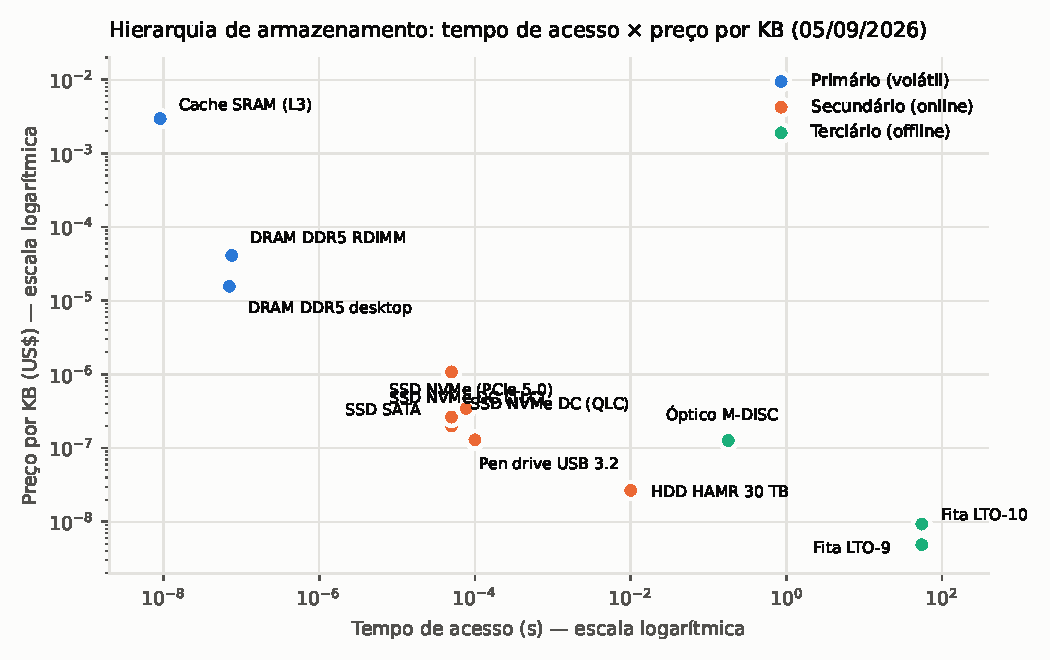
\includegraphics[width=0.92\textwidth]{fig/fig1_hierarquia.pdf}
\caption{Cada tecnologia da Tabela~16.1 atualizada posicionada por tempo de acesso e preço
por kilobyte (ambos em escala logarítmica). A fronteira desce da esquerda superior para a
direita inferior: pagar mais compra latência menor. Note o \textbf{vazio de cinco ordens de
grandeza no eixo horizontal} entre a DRAM ($\sim$10\textsuperscript{-7}\,s) e o SSD NVMe
($\sim$5\,$\times$\,10\textsuperscript{-5}\,s) --- exatamente a lacuna que o Intel Optane
ocupava e que sua descontinuação reabriu.}
\end{figure}

\subsection{Volatilidade e a exigência de durabilidade}

A distinção volátil/não volátil não é um detalhe de engenharia: é a fundação da propriedade
\textbf{D} (\emph{durability}) do ACID. Um \texttt{COMMIT} só pode ser reconhecido ao
cliente depois que os dados de recuperação alcançaram um meio que sobrevive a uma queda de
energia. Toda a arquitetura de \emph{log} de escrita antecipada existe para tornar essa
travessia barata: em vez de escrever páginas de dados espalhadas, escreve-se um registro
sequencial pequeno em um meio persistente.

A consequência prática é que o parâmetro mais importante de um dispositivo, para um SGBD
transacional, não é sua largura de banda, mas a \textbf{latência de uma escrita sincronizada
pequena} --- o custo de um \texttt{fsync}. Voltaremos a esse ponto quantitativamente na
Seção~5.4.

\subsection{Disco magnético: a mecânica que define os parâmetros clássicos}

O disco rígido é o único componente eletromecânico no caminho de dados de um computador
moderno, e sua física dita os quatro parâmetros que aparecem em todo modelo de custo de
SGBD:

\begin{itemize}
\item \textbf{Tempo de busca} (\emph{seek time}) --- deslocamento do braço até a trilha
      correta. Silberschatz reporta faixa de 2 a 20\,ms conforme a distância, com médias
      atuais entre 4 e 10\,ms. O tempo médio de busca é aproximadamente metade do máximo.
\item \textbf{Latência rotacional} --- espera até que o setor desejado passe sob a cabeça.
      É, em média, meia rotação. Um disco \emph{nearline} de 7.200\,rpm gira em 8,33\,ms,
      portanto tem \textbf{4,16\,ms} de latência rotacional média ($60/7200/2 = 4{,}17$\,ms; a
      Seagate publica 4,16) --- valor que a Seagate
      publica explicitamente no manual do Exos~M.
\item \textbf{Taxa de transferência} --- 50 a 200\,MB/s segundo Silberschatz (2018); os
      discos HAMR de 2026 chegam a 275--285\,MB/s sustentados nas trilhas externas, e
      significativamente menos nas internas, que têm menos setores por trilha.
\item \textbf{IOPS} --- número de acessos aleatórios por segundo. Com blocos de 4\,KB,
      Silberschatz reporta 50 a 200\,IOPS. Esse número praticamente \textbf{não melhorou}
      em duas décadas, porque é governado pela mecânica, não pela densidade de gravação.
\end{itemize}

\destaque{O ponto que os livros-texto não enfatizam o bastante}{%
A capacidade do HDD cresceu de 8\,TB (Tabela~16.1 original, 2014) para 32--36\,TB (2026),
um fator de 4$\times$. A taxa sequencial cresceu de 200 para 285\,MB/s, um fator de
1,4$\times$. E o IOPS aleatório \textbf{ficou constante}. O resultado é que o \emph{tempo
para ler o disco inteiro} piorou: varrer 8\,TB a 200\,MB/s levava 11 horas; varrer 32\,TB a
285\,MB/s leva 31 horas. Isso tem consequência direta em SBD: janelas de \emph{backup},
tempo de reconstrução de RAID e viabilidade de \emph{full table scan} degradaram, não
melhoraram. É a principal razão pela qual RAID~5 clássico deixou de ser recomendado para
discos de alta capacidade --- a probabilidade de um segundo erro durante uma reconstrução
de 31 horas deixou de ser desprezível.}

\subsection{Memória flash e SSD: por que a escrita é diferente da leitura}

A memória \emph{flash} NAND é organizada em \textbf{páginas} (tipicamente 4\,KB, análogas a
setores) agrupadas em \textbf{blocos de apagamento} (\emph{erase blocks}) de 256\,KB a
1\,MB, contendo 128 a 256 páginas. A assimetria fundamental é esta:

\begin{itemize}
\item \textbf{Ler} uma página: dezenas de microssegundos.
\item \textbf{Escrever} uma página \emph{previamente apagada}: $\approx$100\,\textmu s.
\item \textbf{Sobrescrever} uma página: \textbf{impossível}. É preciso apagar o bloco
      inteiro, operação que leva 2 a 5\,ms e consome um dos 10\textsuperscript{5} a
      10\textsuperscript{6} ciclos de vida daquele bloco.
\end{itemize}

Essa impossibilidade explica todo o resto da arquitetura de um SSD. A
\textbf{\emph{Flash Translation Layer} (FTL)} mantém um mapeamento dinâmico de páginas
lógicas para páginas físicas: ao atualizar uma página lógica, o controlador escreve em uma
página física já apagada e marca a antiga como inválida. Periodicamente, um processo de
\emph{garbage collection} copia as páginas ainda válidas de um bloco quase vazio para outro
lugar e apaga o bloco. O \textbf{\emph{wear leveling}} distribui os apagamentos
uniformemente, alocando dados ``frios'' aos blocos mais desgastados e dados ``quentes'' aos
menos desgastados. Acima da FTL, o SSD apresenta exatamente a mesma interface orientada a
blocos de um disco magnético --- \emph{``file systems and database storage structures can
thus see an identical logical view of the underlying storage structure''} (Silberschatz,
§12.4).

\destaque{Três consequências para o projetista de SBD}{%
\textbf{(1)~Amplificação de escrita.} Uma escrita lógica de 4\,KB pode custar bem mais que
4\,KB de escrita física, porque o \emph{garbage collection} move dados. Índices com muitas
atualizações in-place (B\textsuperscript{+}-tree clássica) sofrem mais que estruturas
\emph{append-only} (LSM-tree). Não é coincidência que os SGBDs projetados na era do SSD
(RocksDB, Cassandra, ScyllaDB) usem LSM.\\[3pt]
\textbf{(2)~Latência de cauda.} O \emph{garbage collection} ocorre de forma assíncrona e
imprevisível. A latência mediana de um SSD é excelente; a latência de percentil 99,9 pode
ser dez vezes pior. Um SLA de banco de dados quebra na cauda, não na média.\\[3pt]
\textbf{(3)~Paralelismo interno.} Diferentemente do HDD, o SSD atende \textbf{múltiplas
requisições simultâneas} --- 32 é o valor comumente suportado. Um SSD SATA entrega
$\approx$13\,mil IOPS a QD=1 e $\approx$98\,mil a QD=32. Isso muda o desenho do gerente de
\emph{buffer}: emitir uma requisição de cada vez desperdiça o dispositivo.}

Os fabricantes expressam o desgaste em \textbf{DWPD} (\emph{drive writes per day}, escritas
do disco inteiro por dia ao longo da garantia) ou \textbf{TBW} (\emph{terabytes written}).
Um SSD de datacenter de 0,6~DWPD e 61,44\,TB suporta $\approx$134\,PB escritos ao longo de
cinco anos. Para um SGBD, esse é um parâmetro de dimensionamento tão real quanto a
capacidade: um sistema de \emph{log} intensivo pode esgotar a resistência do dispositivo
antes de esgotar seu espaço.

\subsection{Memória de classe de armazenamento: a promessa e o obituário}

Silberschatz dedica a Nota~12.1 à \emph{storage class memory} (SCM): memórias não voláteis
endereçáveis por byte, que evitam a granularidade de página e o custo de apagamento da NAND.
O exemplo citado é o \textbf{3D~XPoint} da Intel/Micron, comercializado como Intel Optane a
partir de 2017 em formato SSD e, a partir de 2018, como módulos de memória persistente
(PMem) instalados em soquetes DIMM.

\correcao{Atualização crítica: a categoria foi extinta comercialmente}{%
A Intel anunciou a saída do negócio Optane em \textbf{julho de 2022}. A geração 300-series
(\emph{Crow Pass}) foi cancelada e nunca chegou ao mercado; os últimos embarques dos
módulos PMem 200-series estavam previstos para o \textbf{fim de 2025}. Em setembro de 2026
\textbf{não existe memória persistente byte-endereçável de propósito geral em produção
corrente}. O degrau da hierarquia descrito na Nota~12.1 do livro-texto simplesmente
desapareceu, reabrindo um vazio de cerca de três ordens de grandeza entre a DRAM
($\approx$70\,ns) e o SSD NVMe mais rápido ($\approx$20--70\,\textmu s).}

O substituto parcial é o \textbf{CXL} (\emph{Compute Express Link}), que não é uma memória,
mas um protocolo coerente sobre a camada física do PCIe. Um módulo CXL Tipo~3 (por exemplo
o Samsung CMM-D MD220, de 256\,GB em formato E3.S, sobre PCIe~Gen5) expõe DRAM adicional ao
sistema operacional com semântica de \emph{load/store}.

A latência é o parâmetro decisivo aqui, e é preciso rigor: \textbf{a Samsung não publica
latência do CMM-D}. O único valor que a empresa divulga no ecossistema CXL é
\textbf{596\,ns}, e refere-se ao CMM-B --- a caixa com \emph{switch}, não o módulo. Medições
independentes revisadas por pares em expansores CXL 2.0 reais situam a latência ociosa entre
\textbf{214 e 271\,ns}, contra 111--117\,ns da DDR5 local no mesmo experimento. Adotamos essa
faixa medida: o CXL custa, portanto, cerca de \textbf{2 a 2,5$\times$ a latência da DRAM
local} --- e não os $\approx$140\,ns que circulam em material promocional. O CXL não
substitui a DRAM: é um \textbf{nível intermediário de memória}, e é por
isso que a especificação CXL~3.2 (dezembro de 2024) introduziu a \emph{Hot-Page Monitoring
Unit}, que permite ao SO ou ao SGBD promover páginas quentes para a DRAM local e rebaixar
as frias para o CXL. Para um SGBD, mais memória barata significa \emph{buffer pool} maior e,
portanto, menos I/O --- o que faz do CXL a tecnologia de infraestrutura mais relevante para
bancos de dados nesta década.

\subsection{Mídia óptica e fita: o estrato terciário em 2026}

O tratamento dos livros-texto envelheceu de forma assimétrica nesses dois meios.

\textbf{Óptico.} Ambos os livros descrevem CD, DVD e Blu-ray como meio de arquivamento
WORM. Em 2026 a categoria está em colapso comercial: em maio de 2025 a Pioneer encerrou, após 45
anos, a fabricação de \textbf{drives ópticos para PC} (o negócio PDDM foi vendido à chinesa
Shanxi Lightchain; a linha de \emph{players} Blu-ray de mesa já havia sido descontinuada por
volta de 2020), e a Sony encerrou toda a linha \emph{Optical Disc Archive} em 31~de~março
de~2025. Sobrevive apenas o nicho de arquivamento WORM de longuíssimo prazo, representado
pelo M-DISC BD-XL de 100\,GB, cuja mídia gravada tem durabilidade declarada de séculos ---
atributo que nenhum outro meio oferece e que interessa a requisitos legais de retenção.

\textbf{Fita.} Aqui os livros subestimam a vitalidade da tecnologia. Silberschatz cita
capacidades de 1 a 12\,TB; a Tabela~16.1 original cita 2,5 a 8,5\,TB. Em 2026 o padrão
corrente é o \textbf{LTO-10}, cuja especificação foi liberada para licenciamento em agosto
de 2025 com \textbf{30\,TB nativos}, e cujo cartucho de \textbf{40\,TB nativos} entrou no
\emph{roadmap} em novembro de 2025, foi anunciado pela Fujifilm em dezembro e começou a ser
embarcado em janeiro de 2026 --- compatível com os \emph{drives} já instalados, sem troca de
hardware, graças a um filme-base de aramida mais fino que permite mais fita no mesmo
cartucho. A taxa nativa de 400\,MB/s supera a de um disco magnético, e o custo da mídia, em
torno de \textbf{US\$\,5 a 10 por TB}, é uma ordem de grandeza inferior ao do HDD.

\correcao{Duas armadilhas do \emph{roadmap} do LTO --- e por que caímos na segunda}{%
\textbf{(1) A taxa não mudou.} O LTO-10 entrega os mesmos \textbf{400\,MB/s nativos} do
LTO-9. A geração 10 ganhou apenas densidade, não velocidade --- o que reforça o argumento da
Seção~2.3: densidade e desempenho escalam por mecanismos diferentes.\\[4pt]
\textbf{(2) O \emph{roadmap} publicado é em capacidade comprimida, e foi revisado para
baixo.} O LTO Program divulga a coluna comprimida (razão 2,5:1) com o mesmo destaque da
nativa, e em \textbf{novembro de 2025} revisou todas as projeções: o LTO-14 passou de
576\,TB para \textbf{365\,TB nativos} --- os \textbf{$\approx$913\,TB} que circulam são
$365 \times 2{,}5$, ou seja, \textbf{capacidade comprimida}, não nativa. As demais gerações
também caíram: LTO-11 de 72 para 70\,TB, LTO-12 de 144 para 120\,TB, LTO-13 de 288 para
210\,TB. Uma versão anterior deste trabalho apresentava ``913\,TB nativos no LTO-14'',
combinando os dois erros --- número comprimido rotulado como nativo, e a partir de um
\emph{roadmap} já revogado. O erro está registrado como E13 na Seção~9.4.}

\destaque{Por que a fita não morreu}{%
A fita é o único meio da hierarquia cujo \emph{drive} e cuja \emph{mídia} são precificados
separadamente. Isso inverte a economia: um \emph{drive} LTO-10 custa dezenas de milhares de
dólares, mas cada terabyte adicional custa US\$\,5--10. Para arquivamento em escala de
petabytes, esse modelo domina qualquer alternativa. Somam-se três atributos que nenhum meio
\emph{online} oferece: consumo energético nulo quando a mídia está na estante
(\emph{cold storage} literal), imunidade a \emph{ransomware} por desconexão física
(\emph{air gap}), e retenção declarada de 30 anos. Para o SBD, a fita não é armazenamento:
é a última linha de defesa do plano de recuperação de desastres.}

\subsection{RAID e confiabilidade}

Silberschatz dedica a Seção~12.5 ao RAID, cuja motivação é aritmética simples: se o MTTF de
um disco é de 100.000 horas, um arranjo de 100 discos tem MTTF agregado de 1.000 horas ---
cerca de 41 dias. Sem redundância, sistemas de grande porte seriam inoperáveis.

Os níveis relevantes na prática, conforme o próprio livro, são o \textbf{RAID~1}
(espelhamento --- melhor desempenho em escrita, custo de 100\% de \emph{overhead}) e o
\textbf{RAID~5} (paridade distribuída --- 1 disco de \emph{overhead}, mas sofre com a
penalidade de escrita: atualizar um bloco exige ler o bloco antigo, ler a paridade antiga,
calcular e escrever ambos, ou seja, \textbf{quatro operações de I/O por escrita lógica}).
Para um SGBD com \emph{log} intensivo, essa penalidade recai justamente sobre o caminho
crítico, e é a razão pela qual a recomendação clássica separa o \emph{log} (em RAID~1) dos
dados (em RAID~5 ou 10).

Com discos de 30\,TB, o RAID~5 tornou-se contraindicado, como observado na Seção~2.3: o
RAID~6 (dupla paridade) ou esquemas de \emph{erasure coding} distribuídos são hoje o padrão
para capacidades altas.

\subsection{Otimizações de acesso a bloco}

Silberschatz (§12.6) enumera as técnicas que o sistema aplica para reduzir o custo de
acesso; todas continuam válidas em 2026, mas com pesos diferentes:

\begin{itemize}
\item \textbf{\emph{Buffering}} --- manter blocos lidos em memória. \emph{Ganhou}
      importância: a memória cresceu mais que o custo de acessá-la.
\item \textbf{\emph{Read-ahead}} --- ler blocos consecutivos antecipadamente. Continua
      valioso para varreduras sequenciais; irrelevante para acesso aleatório.
\item \textbf{Escalonamento de braço} (algoritmo do elevador) --- \emph{perdeu} sentido em
      SSD, que não tem braço. Continua relevante em HDD de capacidade.
\item \textbf{Organização de arquivos em \emph{extents}} --- \emph{perdeu} importância
      relativa em SSD, mas continua reduzindo metadados e fragmentação.
\item \textbf{\emph{Buffers} de escrita não voláteis (NVRAM)} --- permanece essencial. É o
      mecanismo que permite a uma controladora confirmar uma escrita antes que ela alcance
      a mídia, sem violar a durabilidade. Silberschatz alerta corretamente que reordenar
      escritas \emph{sem} NVRAM pode deixar o banco em estado inconsistente após uma queda.
\end{itemize}

\correcao{Uma armadilha de durabilidade que vale para o hardware de 2026}{%
Um adaptador HBA em modo RAID com \emph{cache} de escrita \textbf{não} protegido por
bateria ou \emph{flash} pode confirmar um \texttt{fsync} antes que o dado seja persistido.
O SGBD acredita que cumpriu a durabilidade; uma queda de energia prova o contrário. O mesmo
vale para muitas pontes USB--SATA, que não implementam corretamente o comando FUA
(\emph{Force Unit Access}). Este é o argumento técnico --- não meramente de desempenho ---
para \textbf{não} colocar dados de produção atrás de uma interface USB.}

% =====================================================================
\section{A Tabela 16.1 Atualizada para 2026}

\subsection{A tabela original e o que se pede}

A Tabela~16.1 de Elmasri \& Navathe, ao final da Seção~16.1.1, resume ``\emph{Types of
Storage with Capacity, Access Time, Max Bandwidth (Transfer Speed), and Commodity Cost}''.
Reproduzimos abaixo o original, cujos preços o próprio livro data de \textbf{2014}:

\begin{center}\footnotesize
\setlength{\tabcolsep}{4pt}
\begin{tabular}{@{}lllll@{}}
\toprule
\textbf{Type} & \textbf{Capacity} & \textbf{Access Time} & \textbf{Max Bandwidth} & \textbf{Commodity Prices (2014)} \\
\midrule
Main Memory --- RAM        & 4\,GB--1\,TB      & 30\,ns     & 35\,GB/s                & US\$100--20\,K \\
Flash Memory --- SSD       & 64\,GB--1\,TB     & 50\,\textmu s & 750\,MB/s            & US\$50--600 \\
Flash Memory --- USB stick & 4\,GB--512\,GB    & 100\,\textmu s & 50\,MB/s            & US\$2--200 \\
Magnetic Disk              & 400\,GB--8\,TB    & 10\,ms     & 200\,MB/s               & US\$70--500 \\
Optical Storage            & 50\,GB--100\,GB   & 180\,ms    & 72\,MB/s                & US\$100 \\
Magnetic Tape              & 2,5\,TB--8,5\,TB  & 10--80\,s  & 40--250\,MB/s           & US\$2,5\,K--30\,K \\
Tape jukebox               & 25\,TB--2,1\,EB   & 10--80\,s  & 250\,MB/s--1,2\,PB/s    & US\$3\,K--1\,M+ \\
\bottomrule
\end{tabular}
\end{center}

O enunciado pede quatro modificações: substituir cada tipo por \textbf{exemplos
comercialmente disponíveis}, atualizar capacidade e faixa de preço, \textbf{segregar a
largura de banda em leitura e escrita} quando a informação existir, e acrescentar a coluna
de \textbf{preço por kilobyte}. Adicionamos, por iniciativa do grupo, uma coluna de
\emph{exemplo comercial} explícito e três linhas novas (memória CXL, SSD NVMe de datacenter
e LTO-10), justificadas na Seção~3.3.

\subsection{Tabela 16.1 atualizada --- consulta em 05/09/2026}

A Tabela~\ref{tab:161} ocupa as duas páginas seguintes, em orientação paisagem. Ela deve ser
lida junto com as notas N1 a N11 que a seguem, nas quais está registrada a origem de cada
número: \emph{datasheet} oficial do fabricante, medição publicada por terceiro, derivação
aritmética nossa (com a conta explicitada) ou estimativa de ordem de grandeza. Onde nenhuma
das quatro categorias se aplicava, a célula traz ``n/d'' em vez de um valor inventado.

Três colunas merecem atenção do leitor. A coluna \textbf{tempo de acesso} mistura grandezas
que diferem por dez ordens de grandeza --- de nanossegundos no \emph{cache} a mais de um
minuto na fita --- e é o eixo que organiza toda a hierarquia. As colunas de \textbf{banda de
leitura} e \textbf{banda de escrita} foram segregadas, conforme pede o enunciado, sempre que
a assimetria é conhecida e publicada; para meios genuinamente simétricos (DRAM, disco
magnético, fita) os dois valores coincidem, e isso é em si uma informação. A coluna
\textbf{preço por KB} é a que torna a hierarquia comparável: ela varre seis ordens de
grandeza, de $3{,}0\times10^{-3}$ na SRAM a $4{,}9\times10^{-9}$ na fita LTO-9 --- uma razão
de \textbf{621 mil vezes} entre o topo e a base ($199 \div 65{.}536$ contra
$87{,}99 \div 1{,}8\times10^{10}$).

\newgeometry{landscape,left=1.6cm,right=1.6cm,top=1.8cm,bottom=1.8cm}
\begin{landscape}
\thispagestyle{empty}
{\footnotesize
\setlength{\tabcolsep}{4pt}
\renewcommand{\arraystretch}{1.25}
\begin{longtable}{@{}>{\RaggedRight\arraybackslash}p{3.4cm}>{\RaggedRight\arraybackslash}p{4.3cm}>{\RaggedRight\arraybackslash}p{2.4cm}>{\RaggedRight\arraybackslash}p{2.3cm}>{\RaggedRight\arraybackslash}p{2.2cm}>{\RaggedRight\arraybackslash}p{2.2cm}>{\RaggedRight\arraybackslash}p{3.1cm}>{\RaggedRight\arraybackslash}p{1.9cm}@{}}
\caption{\textbf{Tabela 16.1 atualizada.} Tipos de armazenamento com capacidade, tempo de
acesso, largura de banda segregada em leitura e escrita, preço de mercado e preço por
kilobyte. Preços de referência consultados em 05/09/2026, durante a escassez de memória e
NAND induzida pela demanda de IA (ver Seção~3.4). Fontes por linha nas notas que seguem a
tabela.}\label{tab:161}\\
\toprule
\textbf{Tipo} & \textbf{Exemplo comercial (2026)} & \textbf{Capacidade} &
\textbf{Tempo de acesso} & \textbf{Banda máx.\ leitura} & \textbf{Banda máx.\ escrita} &
\textbf{Preço (US\$)} & \textbf{Preço/KB (US\$)} \\
\midrule
\endfirsthead
\toprule
\textbf{Tipo} & \textbf{Exemplo comercial (2026)} & \textbf{Capacidade} &
\textbf{Tempo de acesso} & \textbf{Banda máx.\ leitura} & \textbf{Banda máx.\ escrita} &
\textbf{Preço (US\$)} & \textbf{Preço/KB (US\$)} \\
\midrule
\endhead
\bottomrule
\endfoot

\textbf{Cache SRAM (L3)} &
AMD Ryzen 9 9950X3D2 (3D V-Cache) / EPYC 9755 &
96\,MB--512\,MB &
$\approx$9,0\,ns$^{\ddagger}$ \newline (L1 0,71; L2 2,50) &
$\approx$1,4\,TB/s por CCD &
$\approx$1,4\,TB/s &
700--14.800 \newline (preço da CPU) &
$3{,}0\times10^{-3}$ \\

\textbf{DRAM (desktop)} &
Corsair Vengeance DDR5-6000 CL30, kit 2$\times$16\,GB &
16--96\,GB (kit) &
70\,ns efetivo \newline (CAS 10,0\,ns) &
96\,GB/s (2 canais) &
96\,GB/s &
270--1.100 &
$1{,}6\times10^{-5}$ \\

\textbf{DRAM (servidor)} &
RDIMM DDR5-6400 64\,GB (Kingston / A-Tech) &
32--256\,GB por módulo &
$\approx$75\,ns &
51,2\,GB/s por módulo \newline (614\,GB/s por soquete, 12 canais) &
51,2\,GB/s &
1.000--4.000 por módulo &
$4{,}2\times10^{-5}$ \\

\textbf{Memória CXL 2.0 (Tipo 3)} \emph{[linha nova]} &
Samsung CMM-D MD220 (E3.S, PCIe Gen5) &
128--256\,GB &
214--271\,ns$^{\dagger}$ \newline (2--2,5$\times$ a DRAM local) &
36\,GB/s &
36\,GB/s &
não público \newline (canal OEM) &
n/d \\

\textbf{SSD NVMe PCIe 5.0 (consumidor)} &
Samsung 9100 PRO 1\,TB (M.2 2280) &
1--8\,TB (dados: 1\,TB) &
$\approx$50\,\textmu s (4\,K, QD1) &
14,7\,GB/s \newline (1,85\,M IOPS) &
13,3\,GB/s \newline (2,60\,M IOPS) &
219,99 (1\,TB, MSRP) &
$2{,}20\times10^{-7}$ \\

\textbf{SSD NVMe \emph{datacenter} QLC} \emph{[linha nova]} &
Solidigm D5-P5336 (U.2 / E3.S / E1.L) &
7,68--122,88\,TB &
8--10\,\textmu s leitura \newline 9\,\textmu s escrita \newline (típica; QoS: 110 / 40\,\textmu s) &
7,0\,GB/s \newline (900\,K IOPS) &
3,0\,GB/s &
16.246--33.249 \newline (61,44\,TB) &
$2{,}6\times10^{-7}$ \\

\textbf{SSD NVMe \emph{datacenter} TLC} \emph{[linha nova]} &
Micron 9550 PRO (E1.S / U.2, PCIe 5.0) &
7,68--30,72\,TB &
$\approx$80\,\textmu s &
14,0\,GB/s \newline (3,3\,M IOPS) &
10,0\,GB/s &
33.217 (30,72\,TB, lista) &
$1{,}1\times10^{-6}$ \\

\textbf{SSD SATA} &
Samsung 870 EVO (2,5 polegadas) &
250\,GB--4\,TB &
77\,\textmu s leitura \newline 28\,\textmu s escrita &
560\,MB/s &
530\,MB/s &
345 (1\,TB) &
$3{,}4\times10^{-7}$ \\

\textbf{Pen drive USB} &
Kingston DataTraveler Max (USB 3.2 Gen 2) &
256\,GB--1\,TB &
$\approx$0,1--0,5\,ms &
1.000\,MB/s &
900\,MB/s &
130 (1\,TB) &
$1{,}3\times10^{-7}$ \\

\textbf{Disco magnético HAMR} &
Seagate Exos M 30\,TB (ST30000NM004K) &
24--36\,TB \newline (44\,TB anunciado) &
$\approx$12,7\,ms \newline (4,16\,ms rot. $+$ $\approx$8,5\,ms busca) &
275\,MB/s sustentado &
275\,MB/s &
800 (30\,TB) --- 1.280 (32\,TB) &
$2{,}7\times10^{-8}$ \\

\textbf{Óptico WORM} &
Verbatim M-DISC BD-XL 100\,GB $+$ Pioneer BDR-X13U &
100\,GB por disco &
$\approx$150--250\,ms &
não publicada \newline ($\approx$36\,MB/s no leitor, 8$\times$) &
$\approx$18\,MB/s (4$\times$) &
12,70 por disco \newline $+$ 230 (leitor) &
$1{,}3\times10^{-7}$ \\

\textbf{Fita LTO-9} &
Cartucho LTO-9 Ultrium (HPE / Fujifilm / IBM) &
18\,TB nativo \newline (45\,TB comp.) &
25--121\,s \newline (carga $+$ \emph{locate}) &
400\,MB/s nativo \newline (1.000 comp.) &
400\,MB/s nativo &
88 por cartucho \newline $+$ 4\,K--6\,K (\emph{drive}) &
$4{,}9\times10^{-9}$ \\

\textbf{Fita LTO-10} \emph{[linha nova]} &
Cartucho LTO-10 Ultrium (Fujifilm, jan./2026) &
30\,TB $\rightarrow$ 40\,TB nativo &
25--121\,s &
400\,MB/s nativo \newline (1.200 comp., FC) &
400\,MB/s nativo &
260--300 por cartucho \newline $+$ $\approx$24\,K (\emph{drive}) &
$9{,}3\times10^{-9}$ \\

\textbf{\emph{Tape library}} &
IBM TS4500 (23.170 cartuchos) / Quantum Scalar i6000 &
até 926,8\,PB nativo \newline (2,317\,EB a 2,5:1) &
25--121\,s &
$\approx$51,2\,GB/s agregado (128 \emph{drives}) &
$\approx$51,2\,GB/s &
sob cotação \newline (não publicado) &
n/d \\
\end{longtable}
}
\end{landscape}
\restoregeometry

\subsubsection*{Notas de rodapé da Tabela~\ref{tab:161}}

\begin{enumerate}[label=\textbf{N\arabic*.},leftmargin=*]
\item \textbf{Preço por KB --- método.} Calculado como (preço do produto) $\div$ (capacidade
      em KB), usando 1\,KB $=$ 2\textsuperscript{10}\,B para SRAM e DRAM e 1\,KB $=$
      10\textsuperscript{3}\,B para os demais. Exemplo verificável (SRAM): o Ryzen 9
      9950X3D2 (192\,MB de L3, US\$\,899) e o 9950X3D (128\,MB, US\$\,700) diferem em
      US\$\,199 por 64\,MiB adicionais, ou seja, US\$\,199\,/\,65.536\,KiB $=
      3{,}04\times10^{-3}$ por KB.
\item \textbf{O preço da SRAM é um \emph{proxy}, não um preço.} Cache SRAM não é vendida
      como produto; o valor acima é o \emph{delta} de preço entre duas CPUs idênticas com e
      sem V-Cache empilhado. Embute margem, custo de empacotamento 3D e segmentação de
      mercado, e deve ser lido apenas como ordem de grandeza --- que é, ainda assim,
      $\approx$80$\times$ o preço por byte da DRAM de servidor.
\item \textbf{Tempo de acesso do \emph{cache} ($\ddagger$) --- derivação, não
      especificação.} Nenhum
      fabricante publica latência de \emph{cache} em nanossegundos; publicam-se ciclos, e
      mesmo esses de forma incompleta. O único valor primário do Zen~5 é
      \textbf{L1D $=$ 4 ciclos} (AMD, Hot Chips 2024). Para o L3, a AMD divulgou apenas um
      \emph{delta}: ``3,5 ciclos a menos'' que o Zen~4, cujo L3 a própria AMD documentou em
      50 ciclos --- donde os $\approx$46{,}5 ciclos que usamos. O L2 de 14 ciclos é número
      do \textbf{Zen~4}: a AMD não republicou o valor para o Zen~5.
      A conversão para nanossegundos exige declarar o \emph{clock}, o que raramente se faz.
      Adotamos o \emph{boost} oficial de até 5,6\,GHz do 9950X3D2:
      $4/5{,}6 = 0{,}71$\,ns (L1), $14/5{,}6 = 2{,}50$\,ns (L2) e
      $46{,}5/5{,}6 = 8{,}30$\,ns (L3), com $+$4 ciclos ($+0{,}71$\,ns) para o V-Cache
      empilhado, totalizando $\approx 9{,}02$\,ns. \textbf{Nenhum desses valores é
      especificação}; todos são derivações declaradas.
\item \textbf{Tempo de acesso do SSD --- e uma distinção que se confunde com frequência.}
      Nenhum fabricante de SSD de \emph{consumo} publica latência em \emph{datasheet}; o
      valor de $\approx$50\,\textmu s do 9100 PRO é estimativa de ordem de grandeza para a
      classe TLC PCIe~5.0. Os SSDs de \emph{datacenter}, ao contrário, publicam --- mas
      publicam \textbf{duas famílias de números que não devem ser trocadas}:
      \begin{itemize}
      \item \textbf{Latência típica} (4\,KB, QD$=$1): 8--10\,\textmu s de leitura e
            $\approx$9\,\textmu s de escrita no D5-P5336. É a latência do caminho de dados
            em regime normal, e é o número comparável com os 214--271\,ns do CXL e os
            $\approx$12,7\,ms do HDD.
      \item \textbf{QoS de percentil} (99,9\% ou 99,99\%): 110\,\textmu s de leitura e
            40\,\textmu s de escrita no mesmo produto. Descreve a \emph{cauda} --- o efeito
            do \emph{garbage collection} discutido na Seção~2.4 --- e não a operação típica.
      \end{itemize}
      A Tabela~\ref{tab:161} traz a latência típica, com o valor de QoS entre parênteses.
      Uma versão anterior deste trabalho apresentava os 110\,\textmu s como ``latência de
      leitura publicada'', confundindo as duas famílias --- erro registrado como E18 na
      Seção~9.4. A ironia é que o QoS é justamente o número que o texto usa como argumento
      na Seção~2.4 (``a mediana é excelente; o P99,9 pode ser dez vezes pior''): 110 contra
      8--10\,\textmu s é exatamente o fator de dez.
\item \textbf{Tempo de acesso do SSD SATA.} Derivado do inverso dos IOPS a QD$=$1
      publicados no \emph{datasheet} do 870 EVO: $1/13.000 \approx 77$\,\textmu s de leitura
      e $1/36.000 \approx 28$\,\textmu s de escrita. A escrita é \emph{mais rápida} que a
      leitura porque é absorvida pelo \emph{cache} SLC (\emph{TurboWrite}).
\item \textbf{Tempo de acesso do HDD.} A Seagate \textbf{removeu o tempo de busca} do
      \emph{datasheet} e do manual do Exos~M. Apenas a latência rotacional (4,16\,ms) é
      publicada. Somamos a ela a busca média típica da classe \emph{nearline} 7.200\,rpm
      ($\approx$8,5\,ms), obtendo $\approx$12,7\,ms --- valor consistente com os 10\,ms da
      Tabela~16.1 original, que mantivemos como referência conforme autoriza o enunciado.
\item \textbf{Bandas de leitura e escrita da fita} referem-se a \emph{drives} de altura
      integral (\emph{full-height}). Unidades de meia altura entregam 300\,MB/s nativos no
      LTO-9. As taxas ``comprimidas'' assumem razão 2,5:1, que é a convenção do LTO Program
      e \textbf{não é atingida} por dados já comprimidos ou cifrados.
\item \textbf{\emph{Tape jukebox}.} Nem a IBM nem a Quantum publicam \emph{throughput}
      agregado. O valor apresentado é derivação nossa: 128 \emph{drives} $\times$ 400\,MB/s
      nativos $=$ 51,2\,GB/s, e representa um teto teórico. Do mesmo modo, a capacidade de
      926,8\,PB é derivada de 23.170 cartuchos $\times$ 40\,TB; a capacidade de
      2,317\,EB é um cenário a 2,5:1, não uma garantia para dados comprimidos/cifrados. Preços de bibliotecas de fita
      são exclusivamente sob cotação.
\item \textbf{Divergência entre rastreadores de preço.} Rastreadores automatizados de preço
      divergem entre si por fatores de até 8$\times$ para DRAM de servidor, conforme puxem
      de \emph{marketplace} ou de distribuidor. Onde havia divergência, adotamos a faixa e
      não um ponto.
\item \textbf{Os números do 9100 PRO são do modelo de 1\,TB}, cuja capacidade e MSRP oficial
      de lançamento (US\$\,219,99) formam a base de cálculo da coluna de preço/KB. O
      \emph{datasheet} Rev.~1.0 mostra
      que a família não é homogênea: o modelo de 4\,TB atinge \textbf{14.800\,MB/s} de
      leitura e \textbf{2.200\,KIOPS} aleatórios de leitura, contra 14.700\,MB/s e
      1.850\,KIOPS do 1\,TB (a escrita é igual em ambos: 13.300--13.400\,MB/s e
      2.600\,KIOPS). Misturar capacidades numa mesma linha --- preço de uma, desempenho de
      outra --- é um erro fácil de cometer e trivial de detectar; por isso a coluna de
      capacidade indica explicitamente de qual modelo vêm os números.
\item \textbf{Latência do módulo CXL ($\dagger$).} \textbf{A Samsung não publica latência
      do CMM-D.} O único valor que a empresa divulga no ecossistema CXL é 596\,ns, e refere-se
      ao CMM-B (a caixa com \emph{switch}), não ao módulo. A faixa de \textbf{214--271\,ns}
      apresentada vem de medições independentes revisadas por pares em expansores CXL 2.0,
      contra 111--117\,ns de DDR5 local no mesmo experimento. Também não é publicada a
      largura de banda agregada do MD220: os 36\,GB/s são estimativa nossa a partir do enlace
      (CXL 2.0 sobre PCIe 5.0 entrega 32\,GB/s por direção em $\times$8 e 64\,GB/s em
      $\times$16). Trate ambos os valores como ordem de grandeza, não como especificação.
\item \textbf{Informações não encontradas.} Por transparência acadêmica, registramos o que
      \textbf{não} conseguimos obter em fonte pública: preço de módulos CXL; preço de RDIMM
      DDR5 de 128\,GB (vendido apenas por contrato de longo prazo a hiperescaladores);
      preço de bibliotecas de fita; latência de pen drive; tempo de acesso de leitor
      Blu-ray; IOPS e latência do Samsung PM1743.
\end{enumerate}

\subsection{Duas linhas com informação incompleta --- e por que as mantivemos}

O enunciado pede que se escolham ``dispositivos para os quais sejam fornecidas as
informações listadas nas quatro colunas da tabela''. Duas linhas da
Tabela~\ref{tab:161} \textbf{não cumprem esse requisito}: a memória CXL e a biblioteca de
fita, ambas com ``n/d'' na coluna de preço. O grupo considera que a decisão de mantê-las
precisa ser argumentada no corpo do texto, e não escondida em nota de rodapé.

\textbf{O critério do enunciado é acertado} --- ele evita que a tabela se encha de produtos
escolhidos por serem interessantes e não por serem documentados, que é exatamente o vício
que a Seção~3.1 procura evitar. Aplicá-lo estritamente, porém, produziria uma tabela que
\emph{descreve mal o mercado de 2026} em dois pontos:

\begin{itemize}
\item \textbf{Memória CXL.} É o único degrau novo da hierarquia desde 2014 e o único
      candidato a ocupar o vazio deixado pelo Optane --- que é a tese central deste
      trabalho. Módulos CXL são vendidos exclusivamente por contrato OEM, sem preço público:
      \emph{nenhum} produto da categoria satisfaria o critério. Excluí-la não seria escolher
      um dispositivo melhor documentado; seria omitir a categoria inteira, e com ela o
      argumento.
\item \textbf{\emph{Tape library}.} Está na Tabela~16.1 original (linha ``Tape jukebox'',
      com faixa de US\$\,3\,K a mais de US\$\,1\,M). Mantivemos a linha por fidelidade ao
      original, mas verificamos que nem a IBM nem a Quantum publicam preço --- bibliotecas
      de fita são vendidas exclusivamente sob cotação. Ou seja: a linha correspondente da
      tabela de 2014 provavelmente já usava estimativa, e nós preferimos declarar a lacuna a
      reproduzir um número sem origem.
\end{itemize}

\textbf{Decisão adotada:} manter as duas linhas com ``n/d'' explícito e origem declarada,
em vez de (a)~removê-las, empobrecendo a descrição do mercado, ou (b)~preenchê-las com
estimativa não rastreável, que é precisamente o que o restante deste trabalho critica.
Registramos que isso constitui um \textbf{desvio consciente} do critério do enunciado, e
não um descuido. As demais doze linhas cumprem o critério integralmente.

\subsection{Justificativa das linhas acrescentadas e removidas}

\begin{itemize}
\item \textbf{Acrescentamos ``Memória CXL 2.0''} porque a hierarquia de 2026 tem um degrau
      que não existia em 2014 e que é o único candidato a ocupar o vazio deixado pelo
      Optane. Sem essa linha, o salto de 70\,ns para 50\,\textmu s ficaria inexplicado.
\item \textbf{Desdobramos ``Flash Memory --- SSD'' em três linhas} (consumidor PCIe~5.0,
      datacenter QLC de alta capacidade e datacenter TLC de alto desempenho) porque a
      categoria única do livro esconde uma variação de \textbf{quatro ordens de grandeza em
      capacidade} (1\,TB a 122,88\,TB) e de mais de 5$\times$ em preço por byte. Para um
      SBD, escolher entre QLC de capacidade e TLC de desempenho é uma decisão de projeto,
      não um detalhe.
\item \textbf{Desdobramos a fita em LTO-9 e LTO-10} porque a transição está em curso
      exatamente agora: o LTO-10 foi lançado em 2025 com 30\,TB e teve o cartucho de 40\,TB
      especificado em novembro de 2025, com embarques a partir de janeiro de 2026.
\item \textbf{Não incluímos o Intel Optane}, apesar de ser a linha que faria mais sentido
      teórico, porque \textbf{não é comercialmente disponível} --- o que viola o critério
      C2. Registramos sua ausência como achado, não como omissão.
\item \textbf{Não incluímos o Sony Optical Disc Archive} pela mesma razão: a linha foi
      encerrada em todas as regiões em 31 de março de 2025.
\end{itemize}

\subsection{Análise: o que mudou entre 2014 e 2026}

\subsubsection*{(a) Capacidade cresceu; latência, quase nada}

\begin{center}\small
\begin{tabular}{@{}lrrr@{}}
\toprule
\textbf{Meio} & \textbf{Capacidade 2014} & \textbf{Capacidade 2026} & \textbf{Fator} \\
\midrule
DRAM (módulo/kit)     & 1\,TB (sistema)  & 256\,GB (módulo) / TBs por soquete & $\approx$4--8$\times$ \\
SSD flash             & 1\,TB            & 122,88\,TB                          & $\approx$123$\times$ \\
Pen drive USB         & 512\,GB          & 2\,TB                               & 4$\times$ \\
Disco magnético       & 8\,TB            & 36\,TB                              & 4,5$\times$ \\
Fita (cartucho)       & 8,5\,TB          & 40\,TB                              & 4,7$\times$ \\
\bottomrule
\end{tabular}
\end{center}

Contra isso, o \textbf{tempo de acesso} do disco magnético permaneceu na mesma casa
(10\,ms $\rightarrow$ 12,7\,ms), e o do SSD melhorou apenas de 50\,\textmu s para
$\approx$50\,\textmu s no consumidor. A lição, que vale para todo modelo de custo de SGBD, é
que \textbf{densidade e latência escalam por mecanismos diferentes}: densidade acompanha a
litografia e a física da mídia; latência acompanha a arquitetura do caminho de dados, que
mudou muito menos.

\subsubsection*{(b) A largura de banda foi o que realmente explodiu}

\begin{figure}[H]\centering
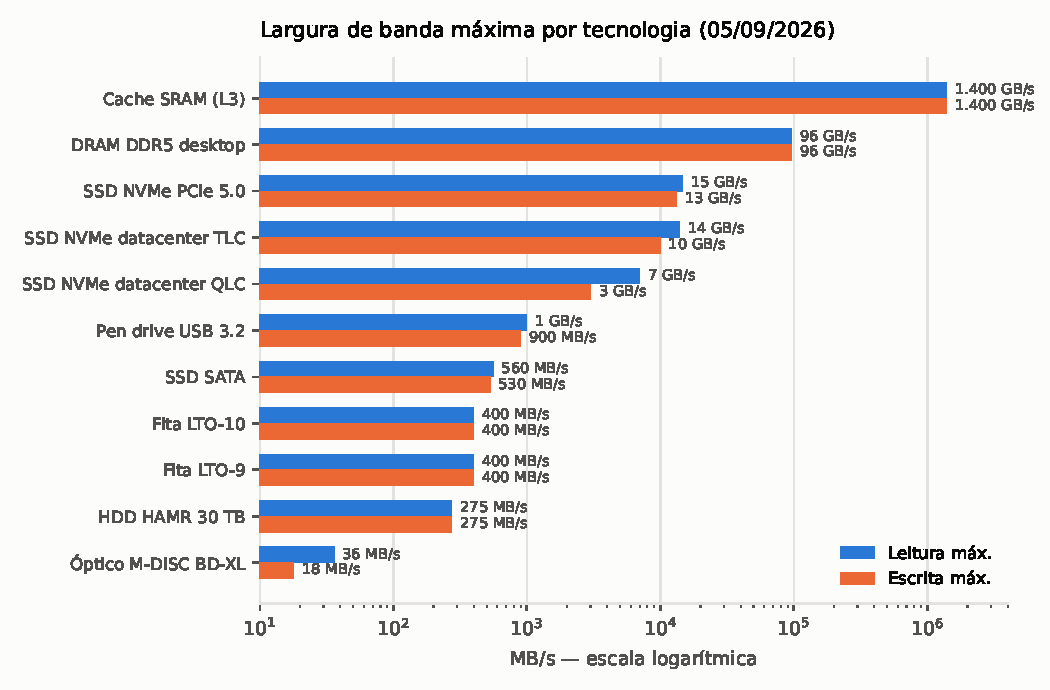
\includegraphics[width=0.92\textwidth]{fig/fig2_banda.pdf}
\caption{Largura de banda de leitura e escrita por tecnologia (escala logarítmica). O SSD
NVMe PCIe~5.0 entrega \textbf{20$\times$} a banda da Tabela~16.1 original para SSD
(750\,MB/s $\rightarrow$ 14,7\,GB/s), enquanto o disco magnético avançou apenas
1,4$\times$. Note que a fita LTO ultrapassa o disco magnético em taxa sequencial --- fato
contraintuitivo que decorre de a fita não precisar posicionar um braço entre blocos
consecutivos.}
\end{figure}

\subsubsection*{(c) SSD e HDD divergiram em vez de convergir}

A expectativa corrente na literatura era de que o preço por terabyte de SSD e HDD
convergisse por volta de 2026--2028. \textbf{O oposto ocorreu.} A razão é estrutural: a
demanda de IA consumiu a capacidade fabril de NAND, e parte dos compradores migrou de SSD
\emph{de volta} para HDD, pressionando também o preço deste.

A razão precisa ser \textbf{datada}, porque é extremamente volátil. O índice de volatilidade
de \emph{flash} da VDURA registra a evolução trimestral do prêmio do SSD corporativo sobre o
HDD \emph{nearline}:

\begin{center}\small
\begin{tabular}{@{}lrrrr@{}}
\toprule
\textbf{Período} & \textbf{3T25} & \textbf{1T26} & \textbf{2T26} & \textbf{3T26 parcial (05/09)} \\
\midrule
Razão SSD/HDD por TB & 7,0$\times$ & 23,2$\times$ (pico) & 16,3$\times$ & \textbf{18,6$\times$} \\
\bottomrule
\end{tabular}
\end{center}

Em agosto de 2026, um SSD TLC corporativo de 30\,TB custava $\approx$US\$\,22.600
($\approx$US\$\,753/TB) contra $\approx$US\$\,1.216 de um HDD de 30\,TB
($\approx$US\$\,41/TB). \textbf{A observação parcial consultada em 05/09/2026 é
18,6$\times$}; ela não deve ser apresentada como fechamento do 3\textsuperscript{o} trimestre.
Os 16,3$\times$ referem-se ao trimestre anterior. Uma versão anterior deste
trabalho citava ``aproximadamente 16$\times$'' sem carimbo de trimestre --- erro registrado
como E15 na Seção~9.4. A lição vale além deste número: em um mercado que oscilou de
7$\times$ a 23$\times$ em quatro trimestres, \textbf{razão sem data não é dado}.

\subsubsection*{(d) A anomalia de preços de 2025--2026}

\correcao{Aviso metodológico obrigatório sobre os preços desta tabela}{%
Os preços da Tabela~\ref{tab:161} foram coletados durante uma \textbf{crise de oferta de
memória e NAND sem precedente}, causada pela realocação de capacidade fabril para HBM
(memória de alta banda para aceleradores de IA) e por pedidos antecipados de
hiperescaladores. Números documentados, cada um com a sua janela: os preços de contrato de
DRAM subiram \textbf{mais de 100\% apenas no 1\textsuperscript{o} trimestre de 2026} para
DRAM de PC (cerca de $+$90\% para DRAM de servidor no mesmo trimestre); o NAND \emph{spot}
subiu cerca de \textbf{5$\times$ entre outubro de 2025 e fevereiro de 2026}, chegando a
8,5$\times$ em março; e o HDD subiu \textbf{46\% em quatro meses}, entre 15 de setembro de
2025 e 14 de janeiro de 2026, em levantamento com doze modelos. Um mesmo kit DDR5-6000 de 32\,GB passou de $\approx$US\$\,80 em meados de 2025
para US\$\,540 na consulta de 05/09/2026 --- alta de $\approx$575\%.\\[4pt]
\textbf{Implicação para a leitura desta tabela:} as \emph{razões} entre tecnologias
(quantas ordens de grandeza separam DRAM de fita) são estruturais e estáveis; os
\emph{valores absolutos} são de um pico anômalo e não devem ser lidos como tendência.
Registramos ainda uma inversão curiosa e temporária: um pen drive USB de 1\,TB
(US\$\,130/TB) está mais barato por terabyte que um SSD SATA de 1\,TB (US\$\,345/TB).}

\subsubsection*{(e) Síntese das mudanças}

\begin{center}\small
\begin{tabular}{@{}p{6.2cm}p{9.0cm}@{}}
\toprule
\textbf{Mudança} & \textbf{Impacto na tabela e no projeto de SBD} \\
\midrule
Optane / 3D XPoint descontinuado (2022--2025) & Removeu o degrau de memória persistente; reabriu vazio de 3 ordens de grandeza entre DRAM e SSD \\
CXL preenche parcialmente o vazio & Novo nível de memória a 214--271\,ns (2--2,5$\times$ a DRAM local); \emph{buffer pool} pode crescer além dos slots DIMM \\
Sony ODA encerrado; Pioneer saiu dos leitores ópticos & Óptico virou nicho de arquivamento WORM de longuíssimo prazo \\
SSD SATA tornou-se legado & Interface satura em 550\,MB/s; mantido só por retrofit \\
PCIe 5.0 é padrão de consumo; PCIe 6.0 chegou ao datacenter & 14,8\,GB/s (consumo) e 28\,GB/s (Micron 9650: anunciado em jul./2025, em produção em massa desde fev./2026) \\
HAMR entrou em produção & HDD saltou de 24\,TB para 32--36\,TB \\
LTO-10 lançado (30\,$\rightarrow$\,40\,TB nativos) & Arquivamento a US\$\,5--10/TB; \emph{roadmap} revisado (nov./2025) até 365\,TB nativos no LTO-14 \\
SSD e HDD divergiram em custo & Razão observada de 18,6$\times$ por TB em 05/09/2026 (3T26 ainda em curso; era 7$\times$ no 3T25) \\
\bottomrule
\end{tabular}
\end{center}

% =====================================================================
\section{Interfaces de Conexão entre o Dispositivo Físico e o Sistema Computacional}

\subsection{Três reduções separam o número de marketing da taxa real}

Antes de qualquer comparação, é preciso fixar a aritmética. Três fatores sucessivos
separam a ``velocidade'' anunciada de uma interface da taxa de dados que ela efetivamente
entrega.

\textbf{(1) Unidade.} 1\,GB/s $=$ 8\,Gb/s. Uma interface de \textbf{6\,Gb/s} nunca entrega
6\,GB/s. Silberschatz, aliás, comete exatamente esse deslize na Seção~12.2 ao escrever que
\emph{``the SATA-3 version of SATA nominally supports 6 gigabytes per second''} --- são
6~\textbf{gigabits} por segundo, como o próprio texto reconhece na frase seguinte ao citar
600\,MB/s.

\textbf{(2) Codificação de linha.} Todo enlace serial insere bits de controle para manter
o balanceamento DC e permitir a recuperação do relógio a partir do próprio fluxo de dados.

\begin{center}\small
\begin{tabular}{@{}lllp{7.4cm}@{}}
\toprule
\textbf{Codificação} & \textbf{Eficiência} & \textbf{\emph{Overhead}} & \textbf{Onde é usada} \\
\midrule
8b/10b        & 80,00\% & 25,0\% & SATA (todas), SAS-1/2/3, PCIe 1.0/2.0, FC 1--8GFC, IB SDR--QDR, USB 3.0 \\
64b/66b       & 96,97\% & 3,1\%  & FC 10/16GFC, IB FDR/EDR, Ethernet 10G$+$ \\
128b/130b     & 98,46\% & 1,6\%  & PCIe 3.0 / 4.0 / 5.0 \\
128b/132b     & 96,97\% & 3,1\%  & USB 3.1/3.2 Gen 2, USB4 Gen3 \\
256b/257b     & 99,61\% & 0,4\%  & FC 32/64/128GFC, IB HDR/NDR/XDR ($+$ RS-FEC) \\
128b/150b     & 85,33\% & 17,2\% & SAS-4 (22,5\,Gb/s) --- inclui FEC embutido \\
FLIT 242B/256B & 94,53\% & 5,5\% & PCIe 6.0 / 7.0 (FLIT mode $+$ RS-FEC $+$ CRC) \\
\bottomrule
\end{tabular}
\end{center}

\textbf{(3) Modulação.} NRZ transmite 1 bit por símbolo. \textbf{PAM4} transmite 2 bits por
símbolo, dobrando a taxa sem dobrar a frequência de sinalização --- ao custo de reduzir a
margem de ruído a um terço, o que torna a correção de erro (FEC) obrigatória. PAM4 é usado
em FC 64/128GFC, InfiniBand HDR/NDR/XDR, PCIe 6.0/7.0 e Ethernet 400G. O USB4 v2.0 usa
\textbf{PAM3} (3 níveis, $\approx$1,58 bit/símbolo).

\destaque{Os dois exemplos canônicos}{%
\textbf{SATA 3.0:} 6,0\,Gb/s bruto $\times$ 8/10 $=$ 4,8\,Gb/s úteis $\div$ 8 $=$
\textbf{600\,MB/s}.\\
\textbf{PCIe 5.0 $\times$4:} 32\,GT/s $\times$ 4 \emph{lanes} $\times$ 128/130 $\div$ 8 $=$
\textbf{15,754\,GB/s}.}

\subsection{Tabela comparativa das interfaces}

\newgeometry{landscape,left=1.4cm,right=1.4cm,top=1.6cm,bottom=1.6cm}
\begin{landscape}
\thispagestyle{empty}
{\scriptsize
\setlength{\tabcolsep}{3.5pt}
\renewcommand{\arraystretch}{1.2}
\begin{longtable}{@{}>{\RaggedRight\arraybackslash}p{2.75cm}>{\RaggedRight\arraybackslash}p{1.1cm}>{\RaggedRight\arraybackslash}p{1.15cm}>{\RaggedRight\arraybackslash}p{2.05cm}>{\RaggedRight\arraybackslash}p{2.15cm}>{\RaggedRight\arraybackslash}p{1.85cm}>{\RaggedRight\arraybackslash}p{1.9cm}>{\RaggedRight\arraybackslash}p{1.1cm}>{\RaggedRight\arraybackslash}p{2.55cm}>{\RaggedRight\arraybackslash}p{2.95cm}@{}}
\caption{\textbf{Comparativo das interfaces de conexão de armazenamento.} Taxas úteis já
descontam a codificação de linha. Latências marcadas com ($\ast$) são estimativas de ordem
de grandeza, sem publicação oficial de organismo normatizador.}\label{tab:if}\\
\toprule
\textbf{Interface} & \textbf{Ano} & \textbf{Ser./Par.} & \textbf{Taxa bruta} &
\textbf{Taxa útil} & \textbf{Latência típ.} & \textbf{Distância máx.} &
\textbf{Hot-plug} & \textbf{Topologia / nº disp.} & \textbf{Uso típico em SBD} \\
\midrule
\endfirsthead
\toprule
\textbf{Interface} & \textbf{Ano} & \textbf{Ser./Par.} & \textbf{Taxa bruta} &
\textbf{Taxa útil} & \textbf{Latência típ.} & \textbf{Distância máx.} &
\textbf{Hot-plug} & \textbf{Topologia / nº disp.} & \textbf{Uso típico em SBD} \\
\midrule
\endhead
\bottomrule
\endfoot

\multicolumn{10}{@{}l}{\textbf{\color{azul}Família USB}}\\
USB 1.0 / 1.1 & 1996/98 & Serial & 1,5 / 12\,Mb/s & 0,19 / 1,2\,MB/s & $\approx$1\,ms$^\ast$ & 3--5\,m & Sim & Estrela hierárq., 127 & Nenhum \\
USB 2.0 (Hi-Speed) & 2000 & Serial & 480\,Mb/s & 60\,MB/s teór.; 30--42 real & 0,2--1\,ms$^\ast$ & 5\,m & Sim & Estrela hierárq., 127 & Mídia de instalação \\
USB 3.0 (3.2 Gen1) & 2008 & Serial & 5\,Gb/s (8b/10b) & 500\,MB/s; $\approx$360 real & 100--200\,\textmu s$^\ast$ & 3\,m & Sim & Estrela hierárq., 127 & \emph{Dump}, exportação \\
USB 3.1 Gen2 (3.2 Gen2) & 2013 & Serial & 10\,Gb/s (128b/132b) & 1.212\,MB/s & $\approx$100\,\textmu s$^\ast$ & 1\,m passivo & Sim & Estrela hierárq., 127 & \emph{Backup} externo \\
USB 3.2 Gen 2$\times$2 & 2017 & Serial 2 \emph{lanes} & 20\,Gb/s & 2.424\,MB/s & $\approx$100\,\textmu s$^\ast$ & 1\,m & Sim & Só USB-C & \emph{Backup} externo \\
USB4 (Gen3$\times$2) & 2019 & Serial 2 \emph{lanes} & 20 / 40\,Gb/s & 2,4 / 4,85\,GB/s & 50--100\,\textmu s$^\ast$ & 0,8\,m passivo & Sim & Roteado (\emph{tunneling}) & SSD externo NVMe \\
USB4 v2.0 & 2022 & Serial PAM3 & 80 (120 opcional/assim.)\,Gb/s & $\approx$9,6\,GB/s nominal & $\approx$50\,\textmu s$^\ast$ & conforme cabo certificado & Sim & Roteado & SSD externo NVMe compatível \\
\midrule
\multicolumn{10}{@{}l}{\textbf{\color{azul}SCSI paralelo (histórico)}}\\
SCSI-1 & 1986 & \textbf{Paralela} 8\,bit & 5\,MB/s & 5\,MB/s & ms$^\ast$ & 6\,m SE / 25\,m HVD & Não & Barramento, 8 IDs & Obsoleto \\
Fast/Wide SCSI-2 & 1994 & \textbf{Paralela} 8/16 & 10 / 20\,MB/s & idem & ms$^\ast$ & 3\,m & Não & Barramento, 8/16 & Obsoleto \\
Ultra160 & 1999 & \textbf{Paralela} 16 & 160\,MB/s & idem & ms$^\ast$ & 12\,m LVD & Não & Barramento, 16 & Obsoleto \\
Ultra-320 & 2002 & \textbf{Paralela} 16 & 320\,MB/s & idem & ms$^\ast$ & 12\,m LVD & Não & Barramento, 16 & Obsoleto \\
\midrule
\multicolumn{10}{@{}l}{\textbf{\color{azul}Família SATA}}\\
SATA 1.0 & 2003 & Serial & 1,5\,Gb/s & 150\,MB/s & 100--200\,\textmu s (SSD) & 1\,m & Sim (AHCI) & Ponto-a-ponto; 15 c/ \emph{port multiplier} & Legado \\
SATA 2.0 & 2004 & Serial & 3,0\,Gb/s & 300\,MB/s & 100--200\,\textmu s & 1\,m & Sim (AHCI) & idem & Legado \\
SATA 3.0--3.5 & 2009--2020 & Serial & 6,0\,Gb/s & \textbf{600\,MB/s} & 100--200\,\textmu s (SSD); 5--10\,ms (HDD) & 1\,m & Sim (AHCI) & idem & Capacidade, \emph{backup}, \emph{dev} \\
eSATA & 2004 & Serial & 3 / 6\,Gb/s & 300 / 600\,MB/s & idem & 2\,m & Sim & Ponto-a-ponto & Obsoleto (sem energia no cabo) \\
eSATAp & $\approx$2009 & Serial & 3 / 6\,Gb/s & idem & idem & 2\,m & Sim & Ponto-a-ponto & Obsoleto \\
SATA Express & 2013 & Serial (PCIe $\times$2) & 10 / 16\,GT/s & 1,0 / 1,97\,GB/s & $<$1\,\textmu s & $\approx$0,3\,m & Sim & Ponto-a-ponto & \textbf{Fracassou} \\
\midrule
\multicolumn{10}{@{}l}{\textbf{\color{azul}Família SAS}}\\
SAS-1 (3G) & 2004 & Serial & 3\,Gb/s (8b/10b) & 300\,MB/s & 100--200\,\textmu s & 10\,m & Sim & \emph{Fabric} c/ \emph{expanders}, 65.535 & Legado \\
SAS-2 (6G) & 2009 & Serial & 6\,Gb/s & 600\,MB/s & idem & 10\,m & Sim & idem & HDD corporativo \\
SAS-3 (12G) & 2013 & Serial & 12\,Gb/s & 1.200\,MB/s & idem & 10\,m & Sim & idem & HDD corporativo \\
SAS-4 (24G) & 2019 & Serial & \textbf{22,5}\,Gb/s (128b/150b) & \textbf{2.400\,MB/s} & idem & 10\,m & Sim & idem & \emph{Backplane} tri-modo \\
\midrule
\multicolumn{10}{@{}l}{\textbf{\color{azul}PCIe e NVMe}}\\
PCIe 3.0 $\times$4 / $\times$16 & 2010 & Serial (\emph{lanes}) & 8\,GT/s por \emph{lane} & 3,94 / 15,75\,GB/s & $<$1\,\textmu s & $\approx$0,3\,m (PCB) & Sim & Árvore ponto-a-ponto & SSD de geração anterior \\
PCIe 4.0 $\times$4 / $\times$16 & 2017 & Serial & 16\,GT/s & 7,88 / 31,51\,GB/s & $<$1\,\textmu s & $\approx$0,3\,m & Sim & idem & SSD de datacenter \\
PCIe 5.0 $\times$4 / $\times$16 & 2019 & Serial & 32\,GT/s & 15,75 / 63,02\,GB/s & $<$1\,\textmu s & $\approx$0,25\,m & Sim & idem & \textbf{Padrão atual} \\
PCIe 6.0 $\times$4 / $\times$16 & 2022 & Serial PAM4 & 64\,GT/s & 30,25 / 121\,GB/s & $<$1\,\textmu s ($+$FEC) & curta & Sim & idem & Fronteira (Micron 9650) \\
PCIe 7.0 $\times$4 / $\times$16 & jun./2025 & Serial PAM4 & 128\,GT/s & 60,5 / 242\,GB/s & $<$1\,\textmu s & curta & Sim & idem & Ainda sem produtos \\
NVMe (local) & 2011--2026 & Protocolo s/ PCIe & --- & $=$ PCIe & \textbf{20--70\,\textmu s} & --- & Sim & 65.535 filas $\times$ 65.536 cmds & \textbf{OLTP, \emph{redo log}} \\
\midrule
\multicolumn{10}{@{}l}{\textbf{\color{azul}\emph{Fabrics} de rede}}\\
NVMe/RoCE v2 & 2016 & \emph{Fabric} Ethernet & 25--400\,GbE & $\approx$ Ethernet & \textbf{41--163\,\textmu s} (P99,99) & $\le$ km & Sim & \emph{Fabric} Ethernet \emph{lossless} & SAN de baixa latência \\
FC-NVMe & 2017 & \emph{Fabric} FC & 32 / 64\,GFC & 3,2 / 6,4\,GB/s & 50--100\,\textmu s$^\ast$ & 10\,km SMF & Sim & \emph{Fabric} FC & SAN corporativa \\
NVMe/TCP & 2018 & \emph{Fabric} IP & 10--400\,GbE & $\approx$ Ethernet & \textbf{122--177\,\textmu s} (P99,99) & roteável; limitada por projeto/SLA & Sim & Rede IP roteável & Alternativa moderna ao iSCSI \\
iSCSI & 2004 (RFC 3720) & Protocolo s/ IP & 1--100\,GbE & 110\,MB/s--11\,GB/s & \textbf{500--800\,\textmu s} & ilimitada (IP) & Sim & Rede IP & PME, virtualização \\
\midrule
\multicolumn{10}{@{}l}{\textbf{\color{azul}FireWire (obsoleto)}}\\
IEEE 1394a (S400) & 1995/2000 & Serial & 400\,Mb/s & $\approx$50\,MB/s & ciclo iso.\ 125\,\textmu s & 4,5\,m (72\,m c/ rep.) & Sim & Árvore/\emph{daisy}, 63 & Descontinuado \\
IEEE 1394b (S800) & 2002 & Serial (8b/10b) & 800\,Mb/s & $\approx$100\,MB/s & idem & 4,5\,m cobre / 100\,m fibra & Sim & 63 & Descontinuado \\
1394-2008 S1600/S3200 & 2008 & Serial & 1,57 / 3,15\,Gb/s & 197 / 393\,MB/s & idem & idem & Sim & 63 & Nunca teve volume \\
\midrule
\multicolumn{10}{@{}l}{\textbf{\color{azul}Fibre Channel}}\\
16GFC (Gen 5) & 2011 & Serial 64b/66b & 14,03\,GBd & 1.600\,MB/s por direção & $\approx$700\,ns/\emph{switch} & 100\,m OM4 / 10\,km & Sim & \emph{Fabric} comutado, $2^{24}$ & SAN legada \\
32GFC (Gen 6) & 2013 & Serial 256b/257b & 28,05\,GBd & \textbf{3.200\,MB/s} & 460\,ns/\emph{switch} & 100\,m OM4 / 10\,km & Sim & idem & \textbf{SAN corporativa} \\
64GFC (Gen 7) & 2020 & Serial PAM4 & 28,9\,GBd $\times$2 & \textbf{6.400\,MB/s} & 460\,ns/\emph{switch} & 100\,m OM4 / 10\,km & Sim & idem & SAN de alto desempenho \\
128GFC (Gen 8) & 2023 & Serial PAM4 & 56,1\,GBd $\times$2 & \textbf{12.425\,MB/s} & idem & 100\,m OM4/OM5 / 10\,km & Sim & idem & Núcleo de SAN \\
FCIP (RFC 3821) & 2004 & Túnel FC s/ TCP/IP & $=$ WAN & $=$ WAN & ms (WAN) & inter-sítios & --- & Túnel sobre IP & Replicação entre \emph{datacenters} \\
FCoE (FC-BB-5) & 2009 & FC s/ Ethernet DCB & 10--40\,GbE & $\approx$ Ethernet & $\approx$ FC $+$ DCB & L2, não roteável & Sim & Ethernet convergente & Nicho/legado em 2026 \\
\midrule
\multicolumn{10}{@{}l}{\textbf{\color{azul}InfiniBand}}\\
IB EDR 4$\times$ & 2014 & Serial 64b/66b & 25,78\,Gb/s por \emph{lane} & 100\,Gb/s & 0,5--1,5\,\textmu s & 100\,m AOC / 10\,km & Sim & \emph{Fabric} comutado & HPC legado \\
IB HDR 4$\times$ & 2018 & Serial PAM4 & 50\,Gb/s por \emph{lane} & 200\,Gb/s & sub-\textmu s & idem & Sim & idem & HPC, IA \\
IB NDR 4$\times$ & 2021 & Serial PAM4 & 100\,Gb/s por \emph{lane} & \textbf{400\,Gb/s} & sub-\textmu s & idem & Sim & idem & Clusters de IA/LLM \\
IB XDR 4$\times$ & 2023 & Serial PAM4 & 200\,Gb/s por \emph{lane} & \textbf{800\,Gb/s} & sub-\textmu s & idem & Sim & idem & Clusters de IA/LLM \\
\midrule
\multicolumn{10}{@{}l}{\textbf{\color{azul}Fatores de forma para NVMe/PCIe} \emph{(conector e mecânica, não protocolo)}}\\
M.2 2280 & 2013 & Serial (PCIe $\times$4) & $=$ PCIe & $=$ PCIe $\times$4 & $=$ NVMe & $\approx$0,1\,m (na placa) & \textbf{Não} & 1 disp.\ por soquete & Boot, cliente, \emph{cache} \\
U.2 (SFF-8639) & 2015 & Serial (PCIe $\times$4) & $=$ PCIe & $=$ PCIe $\times$4 & $=$ NVMe & \emph{backplane} & Sim & 1 disp.\ por baia de 2,5 pol. & Servidor, gaveta frontal \\
U.3 (SFF-TA-1001) & 2019 & Serial (PCIe $\times$4) & $=$ PCIe & $=$ PCIe $\times$4 & $=$ NVMe & \emph{backplane} & Sim & Baia tri-modo: SAS, SATA ou NVMe & Servidor convergente \\
E1.S / E3.S (EDSFF) & 2020 & Serial (PCIe $\times$4/$\times$8) & $=$ PCIe & até $=$ PCIe $\times$8 & $=$ NVMe & \emph{backplane} & Sim & 1 disp.; E3.S~2T aceita módulo CXL & \textbf{Padrão de datacenter} \\
\midrule
\multicolumn{10}{@{}l}{\textbf{\color{azul}Adaptador de barramento} \emph{(categoria de hardware, não protocolo --- ver Seção~4.3.12)}}\\
HBA SAS/SATA/NVMe tri-modo & --- & Placa PCIe & $=$ PCIe 4.0 $\times$8 & 24G SAS por porta & $=$ do meio & \emph{host} & Sim & Ex.: Broadcom eHBA 9600-24i, 24 portas & Modo IT para ZFS, Ceph, réplica por \emph{software} \\
HBA Fibre Channel & --- & Placa PCIe & $=$ PCIe 4.0 $\times$8 & 64GFC por porta & $=$ do \emph{fabric} & \emph{host} & Sim & Ex.: Emulex LPe38102, QLogic 2870 & SAN corporativa, \emph{boot-from-SAN} \\
CNA / HBA iSCSI & --- & Placa PCIe & $=$ Ethernet & $=$ Ethernet & $=$ do \emph{fabric} & \emph{host} & Sim & NIC $+$ \emph{offload} numa porta & \emph{Offload} de iSCSI e NVMe-oF \\
\midrule
\multicolumn{10}{@{}l}{\textbf{\color{azul}Complementares}}\\
Thunderbolt 5 & 2023 & Serial (USB4 v2) & 80 (120 opcional/assim.)\,Gb/s & 64\,Gb/s de PCIe & $\approx$50\,\textmu s$^\ast$ & conforme cabo & Sim & \emph{Daisy-chain}, 6 & SSD externo profissional \\
CXL 3.1 / 3.2 & 2023/24 & Serial (PCIe 6.0) & 64\,GT/s & $\approx$ PCIe 6.0 & 100--250\,ns$^\ast$ & intra-rack & Sim & \emph{Fabric} / \emph{switch} & Expansão de \emph{buffer pool} \\
\end{longtable}
}
\end{landscape}
\restoregeometry

\subsubsection*{Critérios transversais que não cabem em uma taxa de enlace}

\begin{center}\footnotesize
\begin{tabular}{@{}p{2.7cm}p{2.3cm}p{3.0cm}p{3.0cm}p{4.0cm}@{}}
\toprule
\textbf{Classe} & \textbf{Duplex} & \textbf{Portabilidade} & \textbf{Escalabilidade} & \textbf{Confiabilidade/condição} \\
\midrule
USB/Thunderbolt & Bidirecional; banda agregada pode ser assimétrica & Alta, se host, cabo e dispositivo negociam o mesmo modo & Árvore/\emph{daisy-chain}; não é \emph{fabric} de produção & Vazão efetiva e flush/FUA dependem da ponte e do driver \\
SATA/eSATA & Full-duplex lógico & Interno/curta distância & Ponto a ponto; multiplicadores têm limites & Hot-plug depende de AHCI, backplane, firmware e sistema operacional \\
SAS & Full-duplex & Datacenter & \emph{Expanders}, dual-port e muitos dispositivos & Caminhos redundantes e erro fim a fim dependem da implantação \\
PCIe/NVMe local & Full-duplex por \emph{lane} & Interno; formato dependente & Árvore PCIe, filas massivamente paralelas & Hot-plug \textbf{não é universal}: requer suporte de plataforma, firmware, slot/backplane e formato \\
FC/NVMe-oF/iSCSI & Full-duplex & Datacenter/WAN conforme transporte & \emph{Fabric} com múltiplos caminhos & Alta disponibilidade exige duas \emph{fabrics}/redes, MPIO e alvos redundantes \\
\bottomrule
\end{tabular}
\end{center}

\noindent\textbf{Classificação.} USB, SATA, SAS, PCIe, FC, Ethernet e InfiniBand definem
camadas de interconexão; NVMe, iSCSI, FCP, FCIP e FCoE são protocolos/mapeamentos; M.2, U.2,
U.3 e EDSFF são fatores de forma; HBA/CNA são adaptadores. Taxas nominais não devem ser
interpretadas como vazão de aplicação.

\subsubsection*{Como ler as três últimas famílias da Tabela~\ref{tab:if}}

As linhas de \textbf{fatores de forma} (M.2, U.2, U.3, EDSFF) e de \textbf{HBA} são de
natureza distinta das demais e estão incluídas porque constam da lista do enunciado. Elas
\textbf{não são protocolos}: um M.2 não tem ``taxa própria'' --- ele expõe as mesmas
\emph{lanes} PCIe da linha correspondente, e por isso as colunas de taxa trazem ``$=$~PCIe''.
O que distingue essas linhas são as colunas de \textbf{hot-plug}, \textbf{alimentação} e
\textbf{mecânica}, e é aí que estão as decisões de projeto reais: o M.2 não suporta
\emph{hot-swap} e opera só em 3,3\,V, o que limita a dissipação a $\approx$8--11\,W e o
inviabiliza para SSDs PCIe~5.0/6.0 de datacenter, que passam de 25\,W; o EDSFF suporta
\emph{hot-swap}, 12\,V e até 70\,W. Incluí-las na mesma tabela dos protocolos é uma
concessão à lista do enunciado, e o grupo prefere sinalizar a diferença de categoria a
apagá-la.

\subsection{Análise por família}

\subsubsection{USB --- portabilidade máxima, garantias mínimas}

O USB é a interface mais portátil já produzida: \emph{hot-plug} nativo, alimentação pelo
cabo (até 240\,W com Power Delivery 3.1) e até 127 dispositivos por controlador. Duas
observações importam para o estudo.

\textbf{A nomenclatura é deliberadamente confusa.} O USB-IF renomeia retroativamente a cada
revisão: o que foi lançado como USB~3.0 (5\,Gb/s) passou a chamar-se USB~3.1~Gen~1, depois
USB~3.2~Gen~1$\times$1 e, desde 2022, ``USB 5Gbps''. \textbf{É o mesmo silício com três
nomes.} O sufixo \texttt{Gen~N$\times$M} significa: N $=$ geração do transceptor
(velocidade por \emph{lane}); M $=$ número de \emph{lanes}. Assim, Gen~2$\times$2 $=$
2\,\emph{lanes} $\times$ 10\,Gb/s $=$ 20\,Gb/s.

\textbf{USB não serve para dados quentes de SBD} --- e a razão principal \emph{não} é
largura de banda. É que muitas pontes USB--SATA não implementam corretamente o comando FUA
(\emph{Force Unit Access}) nem o \emph{flush} de \emph{cache}, o que compromete a semântica
de barreira de escrita e, portanto, a durabilidade ACID. O USB é adequado para
\emph{backup}, exportação de \emph{dumps} e mídia de instalação.

\subsubsection{SCSI paralelo --- a lição de engenharia que originou tudo}

O SCSI paralelo morreu por uma razão física precisa: o \textbf{\emph{clock skew}}. Em um
barramento paralelo, os bits de uma mesma palavra percorrem trilhas de comprimentos
ligeiramente diferentes e chegam em instantes diferentes. À medida que a frequência sobe, a
janela de amostragem encolhe até desaparecer. O Ultra-640 chegou a ser especificado em 2003,
mas \textbf{nenhum dispositivo foi produzido} --- o cabo teria de encolher para centímetros.

A saída foi \textbf{serializar}: um único par diferencial, com o relógio recuperado do
próprio fluxo de dados, elimina o \emph{skew} entre bits e permite frequências muito mais
altas. Foi assim que nasceram SATA, SAS, PCIe, FC e InfiniBand.

\destaque{O conjunto de comandos sobreviveu ao barramento}{%
O que morreu foi o \emph{barramento} paralelo, não o \emph{protocolo}. O SCSI Command Set
roda hoje sobre SAS, iSCSI, FCP (Fibre Channel Protocol), USB (via UASP) e InfiniBand (via
SRP). É um dos casos mais claros de separação bem-sucedida entre camada física e camada de
comando --- exatamente a separação que o NVMe repetiu ao definir um conjunto de comandos
independente do transporte, executável sobre PCIe, RDMA, TCP ou FC.}

\subsubsection{SATA --- e por que parou em 6\,Gb/s}

O SATA 3.0 é de \textbf{2009} e continua sendo a última mudança de velocidade da família:
dezessete anos de estagnação deliberada. As revisões 3.1 a 3.5 adicionaram apenas recursos
(DevSleep, \emph{Power Disable}, \emph{Rebuild Assist}). Quatro causas convergiram:

\begin{enumerate}
\item \textbf{Custo de engenharia sem retorno.} Dobrar para 12\,Gb/s exigiria requalificar
      conector, cabo, PHY e integridade de sinal de toda a cadeia.
\item \textbf{O \emph{overhead} de 25\% do 8b/10b} é enorme, e trocá-lo por 128b/130b
      quebraria a compatibilidade.
\item \textbf{O gargalo real é o AHCI, não o fio.} O AHCI oferece \textbf{uma} fila de
      \textbf{32} comandos (NCQ), com registradores MMIO que exigem quatro acessos não
      cacheáveis por comando. O NVMe oferece \textbf{65.535 filas de 65.536 comandos},
      uma fila por núcleo, com um único acesso MMIO. Aumentar a banda do SATA sem trocar o
      AHCI não resolveria nem latência nem IOPS.
\item \textbf{O PCIe já existia}, já era mais rápido e já era mais barato por GB/s.
\end{enumerate}

\correcao{Correção a uma afirmação do enunciado da tarefa: SATA \textbf{não} é NL-SAS}{%
O enunciado afirma que ``SATA também é conhecida como NL-SAS''. Esta afirmação é
\textbf{factualmente incorreta}, e o grupo julga importante registrá-la.\\[4pt]
\textbf{NL-SAS} (\emph{Nearline SAS}) designa um disco que combina a \textbf{mecânica, a
mídia, as cabeças e a rotação de 7.200\,rpm de um disco SATA corporativo} com a
\textbf{interface elétrica e o protocolo SAS}. Não é outro nome para SATA: é um terceiro
produto, distinto tanto do SATA quanto do SAS corporativo de 10\,K/15\,K\,rpm.\\[4pt]
A diferença tem consequência prática de projeto. Um disco NL-SAS tem \textbf{duas portas}
(\emph{dual-port}), permitindo \emph{multipath} ativo/ativo para alta disponibilidade, e
aceita o \textbf{conjunto completo de comandos SCSI} com \emph{tagged command queuing}. Um
disco SATA tem uma única porta e o conjunto ATA com NCQ de 32 comandos. Em um
\emph{backplane} SAS, um disco SATA exige tradução por \textbf{STP} (\emph{Serial ATA
Tunneling Protocol}) ou uma placa \emph{interposer}, e perde o caminho redundante; um
NL-SAS não exige nada disso. Para um SGBD em cluster de alta disponibilidade, essa é
exatamente a diferença entre poder e não poder sobreviver à falha de um controlador.}

\begin{center}\small
\begin{tabular}{@{}p{3.6cm}p{3.5cm}p{3.5cm}p{3.5cm}@{}}
\toprule
 & \textbf{SATA (HDD)} & \textbf{NL-SAS} & \textbf{SAS corporativo} \\
\midrule
Interface / protocolo & SATA / ATA & \textbf{SAS / SCSI} & SAS / SCSI \\
Mídia e rotação & \emph{Nearline} 7.200\,rpm & \emph{Nearline} 7.200\,rpm (a mesma) & 10\,K / 15\,K\,rpm \\
Portas & 1 (\emph{single-port}) & \textbf{2 (\emph{dual-port})} & 2 (\emph{dual-port}) \\
\emph{Multipath} / HA & Não & \textbf{Sim} & Sim \\
Comandos & ATA $+$ NCQ (32) & \textbf{SCSI completo, TCQ} & SCSI completo \\
Exige STP/\emph{interposer} em \emph{backplane} SAS & \textbf{Sim} & Não & Não \\
Taxa de erro irrecuperável (URE) & $10^{-14}$ & $10^{-15}$ & $10^{-16}$ \\
\bottomrule
\end{tabular}
\end{center}

\destaque{Ressalva de rigor sobre a nossa própria correção}{%
``NL-SAS'' \textbf{não é termo normativo do T10}: não aparece nas especificações SAS como
categoria definida. É \textbf{convenção de indústria}, consolidada por fabricantes e
integradores para designar essa combinação de mídia \emph{nearline} com interface SAS. A
correção ao enunciado permanece válida --- SATA e NL-SAS não são a mesma coisa, e a
diferença tem consequência de projeto --- mas o grupo a apresenta como uso de mercado, e não
como definição de norma. Pela mesma razão, o \emph{dual-port} da terceira linha da tabela
está sustentado na documentação de fabricantes de \emph{array} e na literatura de
integração, não no material da Dell citado nas referências, que descreve o ganho de
desempenho e a rotação de 7.200\,rpm mas não menciona a segunda porta.}

\subsubsection{eSATA e SATA Express --- dois fracassos instrutivos}

O \textbf{eSATA} (2004) oferecia a mesma taxa do SATA interno com 2\,m de cabo e conector
robusto, sem tradução de protocolo. Foi extinto por um detalhe: \textbf{não fornecia
alimentação pelo cabo}, exigindo fonte externa mesmo em discos portáteis de 2,5''. O
eSATAp tentou corrigir isso combinando pinos de USB e de eSATA, mas nunca foi ratificado e
era eletricamente incompatível entre fabricantes. O USB 3.0, com banda equivalente,
alimentação embutida e um único conector, encerrou a discussão.

O \textbf{SATA Express} (2013) é um caso ainda mais didático. Nasceu obsoleto: o M.2 e o
NVMe foram publicados no mesmo ano. Oferecia apenas \textbf{$\times$2 \emph{lanes}} PCIe
enquanto M.2 e U.2 ofereciam $\times$4. Exigia um conector enorme empilhado sobre duas
portas SATA legadas, mais cabo de dados largo, mais cabo de alimentação separado --- contra
um M.2 que se aparafusa direto na placa sem cabo algum. Praticamente nenhum SSD SATAe
chegou ao varejo, e as portas desapareceram das placas-mãe.

\destaque{A lição comum aos dois fracassos}{%
Tanto o eSATA quanto o SATA Express tentaram \textbf{preservar compatibilidade legada} ---
o primeiro mantendo o protocolo SATA fora da caixa, o segundo empilhando o conector SATA
--- e por isso ficaram piores que as alternativas que romperam com o legado (USB~3.0 e
M.2/NVMe). É o mesmo padrão que se observa no SATA 3.0 preso ao AHCI: o custo de
compatibilidade acaba maior que o custo de recomeçar.}

\subsubsection{PCIe e NVMe --- por que o NVMe venceu}

A vantagem do NVMe sobre o AHCI/SATA é \textbf{estrutural, não de banda}:

\begin{center}\small
\begin{tabular}{@{}p{5.6cm}p{4.2cm}p{4.6cm}@{}}
\toprule
 & \textbf{AHCI / SATA} & \textbf{NVMe} \\
\midrule
Filas de submissão & 1 & \textbf{65.535} \\
Comandos por fila & 32 & \textbf{65.536} \\
Registradores MMIO por comando & 4 (não cacheáveis) & \textbf{1} \\
Afinidade de núcleo & Não & \textbf{Uma fila por núcleo} --- sem contenção de \emph{lock} \\
Conjunto de comandos & ATA (herdado do disco rotativo) & Enxuto, projetado para \emph{flash} \\
\bottomrule
\end{tabular}
\end{center}

Para um SGBD com alta concorrência, o gargalo do AHCI não são os 600\,MB/s: é o
\emph{lock} na fila única. Cada núcleo que quer emitir I/O disputa a mesma estrutura. O
NVMe elimina essa disputa por construção.

\textbf{Fatores de forma.} O M.2~2280 domina o lado cliente, mas \textbf{não suporta
\emph{hot-swap}} e opera apenas em 3,3\,V, o que limita a dissipação a $\approx$8--11\,W ---
insuficiente para SSDs PCIe~5.0/6.0, que passam de 25\,W. O U.2 (SFF-8639) e o U.3
(\emph{backplane} tri-modo, que aceita SAS, SATA ou NVMe na mesma baia) resolveram isso no
servidor, e estão sendo substituídos pela família \textbf{EDSFF}: E1.S (substitui o M.2 em
1U), E1.L (``régua'', densidade de capacidade), E3.S (sucessor do U.2, $\times$4 ou
$\times$8) e E3.S~2T (até 70\,W, usado para módulos de memória CXL). O EDSFF suporta
\emph{hot-swap} e 12\,V, e projeta-se dominante no datacenter até 2028.

\subsubsection{NVMe over Fabrics, iSCSI e a escolha de \emph{fabric}}

O NVMe-oF leva o conjunto de comandos NVMe para fora da máquina. As medições da Western
Digital sobre a mesma mídia tornam a comparação limpa --- desde que se leia o rótulo certo.
As condições são \textbf{4\,KB aleatório, QD$=$1, um \emph{job}, 20 minutos}, e os valores
publicados são de \textbf{percentil 99,99} (``quatro noves''), \textbf{não médias}:

\begin{center}\small
\begin{tabular}{@{}lrrp{6.0cm}@{}}
\toprule
\textbf{Transporte} & \textbf{Escrita (P99,99)} & \textbf{Leitura (P99,99)} & \textbf{Exigência operacional} \\
\midrule
NVMe/RoCE v2 & 41,22\,\textmu s  & 162,82\,\textmu s & Ethernet \emph{lossless} (PFC/DCB/ECN) configurada corretamente \\
NVMe/TCP     & 122,37\,\textmu s & 177,15\,\textmu s & Qualquer rede IP; nenhuma configuração especial \\
iSCSI        & \multicolumn{2}{c}{500--800\,\textmu s (típica)} & Qualquer rede IP; camada extra de tradução SCSI \\
\bottomrule
\end{tabular}
\end{center}

O \emph{trade-off} é nítido. O RoCE exige rede sem perdas; se o PFC for mal configurado,
produz \emph{congestion spreading} e \emph{head-of-line blocking} --- o pesadelo operacional
clássico de SAN Ethernet. O NVMe/TCP roda em redes IP convencionais e reduz requisitos
operacionais, ao preço de 80--150\,\textmu s adicionais neste ensaio e maior consumo de CPU.
\textbf{Para muitos SBDs que priorizam simplicidade operacional, NVMe/TCP é uma escolha
plausível}; RoCE justifica-se quando P99 abaixo de
150\,\textmu s for requisito duro.

\correcao{Por que insistimos no rótulo ``P99,99''}{%
Os quatro valores acima são frequentemente citados como ``latência do NVMe/TCP'' sem
qualificação --- inclusive por nós, numa versão anterior deste documento (erro E19,
Seção~9.4). A distinção importa por dois motivos. \textbf{Primeiro}, valores de cauda são
tipicamente 2 a 5 vezes maiores que a mediana; comparar um P99,99 de rede com uma latência
típica de dispositivo mistura grandezas e infla artificialmente o custo do \emph{fabric}.
\textbf{Segundo} --- e esta é a razão pela qual mantivemos os números mesmo assim ---
\textbf{para um SBD a cauda é o que importa}: é o P99,9 que quebra um SLA, não o P50. Ou
seja, o número está certo e é o mais relevante; o que faltava era dizer que número ele é.}
O iSCSI permanece consolidado em bases instaladas e ambientes menores; o NVMe/TCP é uma
alternativa mais nova e, no ensaio citado, apresentou menor latência sobre a mesma mídia.

\subsubsection{SAS --- imortal, mas fora da corrida do SSD}

O SAS resolveu tudo o que o SCSI paralelo não conseguia: 10\,m de cabo (dez vezes o SATA),
\emph{fabric} com \emph{expanders} para até \textbf{65.535 dispositivos}, endereço WWN de
64\,bits, \emph{dual-port} nativo e \emph{hot-plug} pleno. Mas perdeu a corrida do SSD por
duas razões admitidas pela própria STA (SCSI Trade Association): o NVMe foi projetado do
zero para \emph{flash}, enquanto o SAS foi otimizado para HDD numa era sem SSD; e o NVMe usa
\textbf{4 \emph{lanes} PCIe} contra 1--2 \emph{lanes} do SAS.

\textbf{Status do SAS-5:} o projeto existe formalmente no T10 como \textbf{BSR INCITS 561,
revisão 04 de 11 de maio de 2026}, em fase de \emph{INCITS Approval / Public Review}, com o
primeiro período de revisão pública encerrando em \textbf{29 de setembro de 2026}. O
documento de projeto \textbf{não publica taxa de enlace}: os 45\,Gb/s que circulam em fóruns
e roteiros de marketing não têm respaldo normativo, e este trabalho não os adota. O que de
fato avança em produto é o 24G$+$ (SAS-4.1), que --- nas palavras do presidente da STA ---
``terá a mesma velocidade física de interface do 24G'', ou seja, \textbf{não há aumento de
velocidade previsto}. O SAS permanece relevante em \textbf{HDDs} corporativos e
\emph{backplanes} tri-modo; sem uma série de mercado datada, não se afirma participação
majoritária.

Registre-se também uma imprecisão de marca: \textbf{``24G SAS'' opera a 22,5\,Gb/s}, não a
24; o número 24 é arredondamento comercial.

\subsubsection{FireWire --- e por que perdeu para o USB}

O IEEE~1394 era tecnicamente superior ao USB da sua época: DMA \emph{peer-to-peer} sem
intervenção da CPU do hospedeiro, 8--45\,W de alimentação a 24--30\,V (contra 2,5\,W do USB
2.0), e 100\,m sobre fibra no 1394b. Perdeu por três motivos: custo de licenciamento e de
silício, a reserva de \textbf{80\% da banda para tráfego isócrono} (foi projetado para vídeo
DV, não para acesso aleatório a blocos), e a própria vantagem do DMA direto, que se revelou
uma \textbf{vulnerabilidade de segurança} (ataques de DMA sobre a porta FireWire).

Está morto: a Apple descontinuou entre 2011 e 2012, removeu o suporte do macOS em 2025; o
Windows não inclui drivers desde o Windows~10.

\subsubsection{HBA --- esclarecimento de categoria}

\correcao{HBA não é uma interface nem um protocolo}{%
O enunciado lista ``HBA'' junto com USB, SATA e SAS, mas HBA (\emph{Host Bus Adapter}) é
uma \textbf{categoria de hardware}, não um padrão de conexão. É a placa (ou o chip
integrado à placa-mãe) que liga o barramento do hospedeiro --- quase sempre PCIe --- a um
barramento ou \emph{fabric} de armazenamento (SAS, SATA, Fibre Channel, Ethernet/iSCSI,
InfiniBand). Ela contém o controlador, os PHYs, memória e o \emph{firmware} que implementa
o protocolo de transporte.}

Três distinções importam para um SBD:

\begin{itemize}
\item \textbf{HBA puro (modo IT, \emph{Initiator Target}) $\times$ controladora RAID.} O HBA
      puro expõe os discos individualmente ao sistema operacional, sem \emph{cache} de
      escrita nem metadados de RAID --- é o que ZFS, Ceph, Storage Spaces e SGBDs com
      replicação por software exigem. A controladora RAID faz RAID em hardware com
      \emph{cache} protegido por bateria ou \emph{flash}.
\item \textbf{HBA $\times$ NIC.} Uma placa de rede comum com iniciador iSCSI em software é
      diferente de um \emph{HBA} iSCSI, que faz \emph{offload} completo em hardware e
      permite \emph{boot-from-SAN}.
\item \textbf{CNA} (\emph{Converged Network Adapter}) combina NIC e HBA FCoE/iSCSI em uma
      única porta Ethernet.
\end{itemize}

Exemplos correntes: Broadcom eHBA 9600-24i (tri-modo SAS/SATA/NVMe, PCIe~4.0, 24G SAS);
Broadcom/Emulex LPe38102 e Marvell/QLogic 2870 (Fibre Channel 64GFC, PCIe~4.0, com FC-NVMe
e FCP concorrentes na mesma porta); NVIDIA ConnectX-7/8 e BlueField-3 (InfiniBand e Ethernet
com \emph{offload} de NVMe-oF).

\subsubsection{Fibre Channel, FCIP e FCoE}

O Fibre Channel domina SANs corporativas de missão crítica por uma propriedade que nenhuma
rede IP oferece nativamente: é \textbf{L2 dedicado com controle de fluxo por \emph{buffer
credits}} --- crédito por \emph{buffer}, não por janela --- ou seja, \textbf{sem perdas por
construção}. Não há retransmissão, não há colapso por congestionamento, não há TCP. Um
\emph{switch} Brocade G720 (Gen~7) entrega \textbf{460\,ns de latência porta a porta}, sob
duas condições que o \emph{product brief} da Broadcom declara e que devem ser citadas
junto: \textbf{portas comutadas localmente} (\emph{locally switched}) e \textbf{já incluindo
o FEC}.

\correcao{Armadilha de leitura das especificações da FCIA}{%
A coluna ``throughput'' do \emph{speedmap} oficial da FCIA é \textbf{full-duplex}, isto é,
a soma das duas direções. Um HBA ``64GFC'' entrega \textbf{6.400\,MB/s por direção}, e não
12.800\,MB/s em uma direção. Adotamos, na Tabela~\ref{tab:if}, a taxa \textbf{por direção},
que é a comparável com as demais interfaces.}

\textbf{FCIP} (RFC 3821) tuneliza FC sobre TCP/IP para estender SANs entre \emph{datacenters}
--- é a forma padrão de fazer replicação de \emph{storage} entre sítios, e continua viva.

\textbf{FCoE} ocupa um nicho legado nas novas implantações. A promessa era convergência (um cabo só), mas exigia
DCB fim a fim (PFC, ETS, DCBX), configuração frágil e cara, e não era roteável em L3. Ficou
espremido: quem precisava de determinismo continuou no FC nativo; quem queria simplicidade
foi para iSCSI e depois NVMe/TCP. Diagnósticos de obituário circulam desde 2015.
\textbf{Atenção à distinção}: a adoção nova de FCoE é limitada;
\textbf{Fibre Channel nativo permanece ativo} --- a
especificação FC-PI-8 (128GFC) foi concluída em 2023 e publicada como INCITS~560-2023, e o
\textbf{256GFC está em desenvolvimento no T11} (FC-PI-9) --- em desenvolvimento, note-se,
não publicado.

\subsubsection{InfiniBand --- o \emph{fabric} da era da IA}

O InfiniBand não é uma interface de disco: é o \emph{fabric} que transporta NVMe-oF/RDMA,
SRP, iSER e, sobretudo, tráfego MPI/NCCL entre GPUs. Sua latência fim a fim é de
\textbf{0,5 a 1,5\,\textmu s} --- uma a duas ordens de grandeza abaixo do TCP/Ethernet
convencional. A razão é arquitetural: RDMA nativo com \textbf{\emph{kernel bypass}} e
\textbf{\emph{zero-copy}} (a placa lê e escreve diretamente na memória da aplicação, sem
chamada de sistema, sem cópia e sem interrupção por pacote), controle de fluxo
crédito-a-crédito sem perdas, e roteamento por um \emph{Subnet Manager} centralizado.

A geração corrente é XDR (800\,Gb/s em 4$\times$, outubro de 2023), com \emph{switches}
NVIDIA Quantum-X800 que executam redução coletiva dentro da rede (SHARP).

\textbf{Relevância para SBD:} o \textbf{GPUDirect Storage} estabelece um caminho de DMA
direto do SSD NVMe (ou da placa de rede, via NVMe-oF) \textbf{para a memória da GPU},
eliminando o \emph{bounce buffer} na memória do hospedeiro. A NVIDIA reporta até
\textbf{8$\times$} de ganho de banda, \textbf{3$\times$} de redução de latência e
\textbf{3$\times$} de melhora no uso de CPU. É a fundação técnica dos bancos acelerados por
GPU (RAPIDS/cuDF, HeavyDB) e dos pipelines de treinamento que leem Parquet direto do
armazenamento.

\textbf{A disputa em aberto:} o \emph{Ultra Ethernet Consortium} publicou a Especificação
1.0 em junho de 2025, definindo uma pilha Ethernet para IA/HPC que ataca as duas fraquezas
do RoCE clássico --- a exigência de \emph{lossless} rígido e a falta de escala em
\emph{incast}. Em 2026 a disputa segue indefinida: o InfiniBand domina os maiores clusters
NVIDIA; a Ethernet/UEC ganha terreno entre hiperescaladores que priorizam multifornecedor.

\subsection{Orçamento de latência ponta a ponta}

A tabela abaixo decompõe uma leitura aleatória de 4\,KB. É, no entendimento do grupo, a
tabela mais útil de todo este trabalho para quem projeta um SBD.

\begin{center}\small
\setlength{\tabcolsep}{4pt}
\begin{tabular}{@{}p{3.6cm}rrrrr@{}}
\toprule
\textbf{Etapa} & \textbf{NVMe local} & \textbf{NVMe/RoCE} & \textbf{NVMe/TCP} & \textbf{iSCSI 10\,GbE} & \textbf{HDD SAS} \\
\midrule
Chamada de sistema $+$ camada de bloco & 2--5\,\textmu s & 2--5\,\textmu s & 5--10\,\textmu s & 10--20\,\textmu s & 5\,\textmu s \\
\emph{Driver} $+$ submissão na fila & 1--2\,\textmu s & 2\,\textmu s & 5\,\textmu s & 20--50\,\textmu s & 10\,\textmu s \\
\textbf{Travessia do barramento/\emph{fabric}} & \textbf{$<$1\,\textmu s} & 5--15\,\textmu s & 50--120\,\textmu s & 200--400\,\textmu s & 5\,\textmu s \\
\textbf{Latência da mídia} & \textbf{20--70\,\textmu s} & 20--70\,\textmu s & 20--70\,\textmu s & 20--70\,\textmu s & \textbf{$\approx$4\,ms} \\
Controladora do alvo / RAID & --- & 10--30\,\textmu s & 10--30\,\textmu s & 30--80\,\textmu s & 50\,\textmu s \\
\midrule
\textbf{TOTAL} & \textbf{20--70\,\textmu s}$^{a}$ & \textbf{41--163\,\textmu s}$^{b}$ & \textbf{122--177\,\textmu s}$^{b}$ & \textbf{500--800\,\textmu s}$^{a}$ & \textbf{5--10\,ms}$^{a}$ \\
\bottomrule
\end{tabular}
\end{center}

\footnotesize $^{a}$~latência típica. \quad $^{b}$~percentil 99,99 medido pela Western
Digital (4\,KB, QD$=$1); a mediana correspondente é menor. As duas colunas de
\emph{fabric} são, portanto, \textbf{conservadoras} em relação às demais --- o que reforça,
e não enfraquece, a conclusão (2) abaixo.\normalsize

\destaque{Três conclusões}{%
\textbf{(1) Em NVMe local, cerca de 90\% da latência é mídia, não protocolo.} O barramento
PCIe custa menos de 1\,\textmu s dentro de um orçamento de 20--70\,\textmu s. Segue-se que
\textbf{migrar de PCIe~5.0 para 6.0 não reduz a latência de leitura aleatória} --- aumenta
banda sequencial e IOPS agregados. Quem quiser cortar latência precisa trocar a
\emph{mídia}, não o barramento. E a mídia que faria isso (SCM/Optane) saiu do mercado.\\[4pt]
\textbf{(2) Em \emph{storage} de rede, o protocolo passa a dominar.} O NVMe/TCP acrescenta
100--150\,\textmu s à \emph{mesma} mídia; o iSCSI acrescenta 400--700\,\textmu s. Aqui,
trocar de protocolo tem efeito de primeira ordem.\\[4pt]
\textbf{(3) A cauda importa mais que a média.} \emph{Garbage collection} do SSD, replicação
e reconstrução criam picos que a média esconde. Um SLA de banco de dados quebra no P99,9,
não no P50. É nesse ponto que \emph{fabrics} sem perdas (FC, InfiniBand, RoCE bem
configurado) vencem o TCP: variância muito menor.}

\begin{figure}[H]\centering
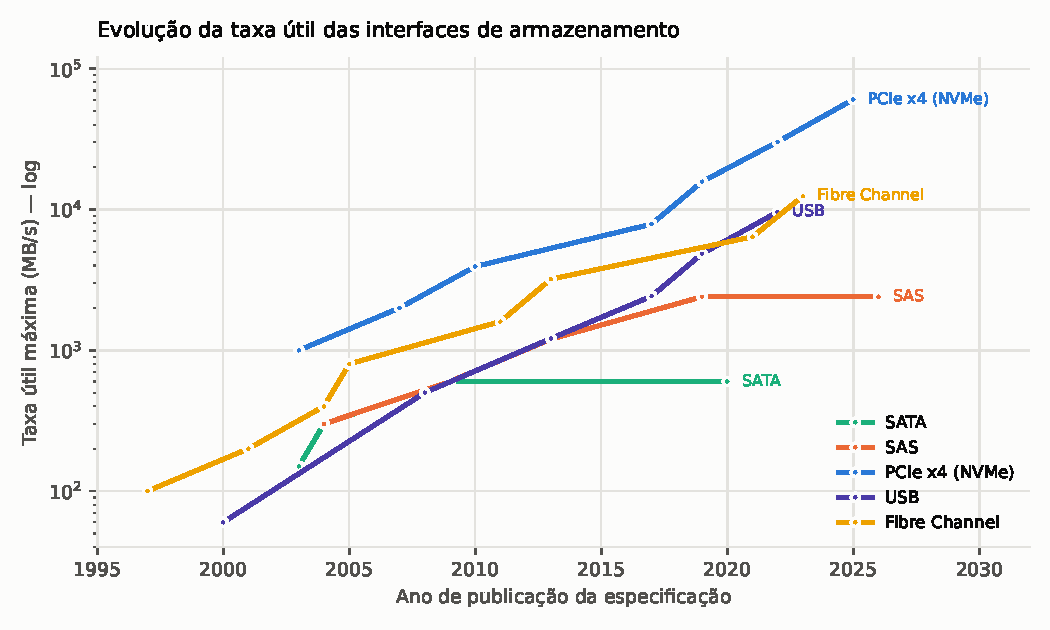
\includegraphics[width=0.92\textwidth]{fig/fig3_interfaces.pdf}
\caption{Evolução da taxa útil máxima das principais famílias de interface, em escala
logarítmica. A linha horizontal do SATA a partir de 2009 é a estagnação discutida na
Seção~4.3.3; o PCIe é a única família cuja inclinação se manteve constante por duas décadas
--- o que explica por que todas as demais interfaces de armazenamento acabaram construídas
sobre ele.}
\end{figure}

% =====================================================================
\section{Implicações para o Gerente de Armazenamento do SBD}

\subsection{O que é o gerente de armazenamento}

Na arquitetura de um SGBD, o \emph{gerente de armazenamento} (\emph{storage manager}) é o
módulo que media entre as estruturas lógicas --- relações, tuplas, índices --- e o meio
físico. Suas responsabilidades incluem a alocação de espaço em arquivos e \emph{extents},
o mapeamento de páginas lógicas para blocos físicos, a gerência do \emph{buffer pool}, a
emissão e o escalonamento de operações de I/O, e a garantia das propriedades de
durabilidade exigidas pelo gerente de transações.

Toda decisão desse módulo é parametrizada por características do dispositivo. Esta seção
converte os números das Seções~3 e~4 em parâmetros acionáveis.

\subsection{Tamanho de bloco e de \emph{extent}}

Silberschatz reporta blocos de 4 a 16\,KB; a página NAND é tipicamente 4\,KB e o bloco de
apagamento, 256\,KB a 1\,MB. Isso produz recomendações distintas por meio:

\begin{center}\small
\begin{tabular}{@{}p{3.0cm}p{2.6cm}p{9.4cm}@{}}
\toprule
\textbf{Meio} & \textbf{Bloco recomendado} & \textbf{Justificativa} \\
\midrule
HDD & 8--64\,KB & O custo é dominado pela busca ($\approx$12,7\,ms); uma vez paga, ler mais é quase de graça (285\,MB/s $\Rightarrow$ 64\,KB custa 0,22\,ms). Blocos maiores amortizam a busca. \\
SSD NVMe & 4--16\,KB & Alinhar à página NAND de 4\,KB evita leitura-modificação-escrita. Blocos maiores desperdiçam banda em acesso aleatório, já que não há busca a amortizar. \\
Fita / arquivamento & $\ge$1\,MB & Meio sequencial; o custo é de posicionamento (25--121\,s). Só faz sentido operar em unidades muito grandes. \\
\bottomrule
\end{tabular}
\end{center}

O conceito de \textbf{\emph{extent}} --- conjunto de blocos consecutivos alocados de uma vez
--- continua útil em SSD, mas por outra razão: não mais para evitar buscas, e sim para
reduzir metadados, melhorar a localidade da FTL e permitir que o \emph{garbage collection}
libere blocos de apagamento inteiros.

\subsection{\emph{Buffer pool}: profundidade de fila é tão importante quanto tamanho}

O gerente de \emph{buffer} foi projetado em uma era em que o dispositivo atendia
\textbf{uma} requisição por vez. Um SSD moderno atende \textbf{32 ou mais} em paralelo, e a
diferença é dramática: um SSD SATA entrega $\approx$13\,mil IOPS a QD$=$1 e $\approx$98\,mil
a QD$=$32; um SSD NVMe passa de 350\,mil leituras aleatórias de 4\,KB por segundo.

\destaque{Consequência de projeto}{%
Um gerente de \emph{buffer} que emite uma falta de página por vez e bloqueia esperando
usa, na melhor das hipóteses, \textbf{3\% da capacidade} de um SSD NVMe. Extrair o
desempenho do dispositivo exige \textbf{I/O assíncrono com múltiplas requisições em voo}
--- \emph{prefetch} agressivo em varreduras, leitura antecipada de nós de índice, I/O
paralelo por \emph{worker}. É exatamente por isso que SGBDs modernos adotaram
\texttt{io\_uring} no Linux e que o PostgreSQL introduziu \emph{I/O assíncrono} em suas
versões recentes. O parâmetro \texttt{effective\_io\_concurrency} do PostgreSQL existe
literalmente para informar ao planejador quantas requisições paralelas o dispositivo
suporta.}

\subsection{Latência de \emph{commit}: o parâmetro mais importante de todos}

Um \texttt{COMMIT} exige um \texttt{fsync} do registro de \emph{log}. Trata-se de um I/O
\textbf{síncrono e pequeno (8--16\,KB)}. Isolando apenas uma escrita e sem \emph{group
commit}, \emph{cache} protegido, paralelismo, FUA ou tempo de CPU, obtém-se o limite
ilustrativo $1/\text{latência do fsync}$; ele \textbf{não} é o throughput previsto do banco.

\begin{center}\small
\begin{tabular}{@{}lp{3.6cm}p{4.4cm}@{}}
\toprule
\textbf{Meio do \emph{log}} & \textbf{Latência de escrita síncrona} & \textbf{Teto teórico de \emph{commits}/s por \emph{thread}} \\
\midrule
HDD 7.200\,rpm (sem NVRAM)   & $\approx$8\,ms       & $\approx$125 \\
SSD SATA                     & $\approx$150\,\textmu s & $\approx$6.700 \\
SSD NVMe local               & $\approx$30\,\textmu s  & $\approx$33.000 \\
NVMe/TCP (remoto)            & $\approx$122\,\textmu s & $\approx$8.200 \\
iSCSI 10\,GbE                & $\approx$600\,\textmu s & $\approx$1.700 \\
SCM / Optane (hipotético)    & $\approx$10\,\textmu s  & $\approx$100.000 \\
\bottomrule
\end{tabular}
\end{center}

Duas leituras deste quadro. Primeira: \textbf{nenhum aumento de largura de banda do SATA
resolveria isso} --- o problema é latência, não vazão, e foi exatamente o que o NVMe atacou
e o AHCI não podia atacar. Segunda: a linha do SCM mostra o que \emph{teria sido possível}
e que a descontinuação do Optane retirou da mesa; é a razão pela qual o desaparecimento
dessa categoria (Seção~2.5) é o achado mais consequente deste trabalho para bancos de dados
transacionais.

A mitigação clássica --- \textbf{\emph{group commit}}, que agrupa vários \texttt{COMMIT}s em
um único \texttt{fsync} --- continua sendo o mecanismo que separa um SGBD que usa o
dispositivo de um que o desperdiça.

\subsection{O modelo de custo do otimizador envelheceu}

O modelo de custo clássico conta \textbf{blocos lidos}. Garcia-Molina, Ullman \& Widom
formalizam essa prática no Capítulo~13 sob o nome de \textbf{\emph{I/O model of
computation}}, cuja premissa é enunciada de forma explícita: \emph{o tempo de uma operação
sobre disco é dominado pelo número de acessos a bloco, e o custo de CPU pode ser
desprezado}. Toda a análise de algoritmos de junção, ordenação externa e varredura da
disciplina repousa sobre essa premissa.

O ponto que este trabalho quer levantar é que \textbf{a premissa tinha uma justificativa
quantitativa, e essa justificativa mudou}. Ela valia porque um acesso a bloco em disco
magnético custava $\approx$10\,ms enquanto uma instrução de CPU custava $\approx$1\,ns ---
sete ordens de grandeza. Com um SSD NVMe a $\approx$50\,\textmu s e CPUs de vários
gigahertz, a distância caiu para cerca de \textbf{quatro ordens de grandeza}, e em cargas
com muitas requisições em paralelo o custo de CPU do próprio caminho de I/O (chamada de
sistema, cópia de \emph{buffer}, tratamento de interrupção --- as duas primeiras linhas da
tabela de orçamento da Seção~4.4) deixou de ser desprezível: em NVMe local ele responde por
5 a 10\,\textmu s dos 20--70\,\textmu s totais. O modelo de I/O não se tornou falso; tornou-se
\textbf{menos dominante}, e o erro que ele induz deixou de ser irrelevante.

O modelo clássico também distingue acesso sequencial de aleatório com uma razão da ordem de
\textbf{1:100} em HDD --- o que justifica a regra prática de que uma varredura completa
(\emph{full table scan}) vence o uso de índice quando a seletividade é pior que
$\approx$5--10\%.

Em SSD NVMe, essa razão cai para algo entre \textbf{1:1 e 1:3}. A consequência direta é que
o \textbf{ponto de equilíbrio entre varredura e índice se desloca substancialmente}: o
índice passa a valer a pena para seletividades muito piores do que a regra clássica sugere.

\destaque{Onde isso aparece na prática}{%
O PostgreSQL expõe esse modelo em dois parâmetros: \texttt{seq\_page\_cost} (padrão 1,0) e
\texttt{random\_page\_cost} (padrão \textbf{4,0}). O valor 4,0 codifica a premissa de disco
magnético. A recomendação corrente para armazenamento SSD é reduzir
\texttt{random\_page\_cost} para \textbf{1,1--1,5}. Não fazê-lo faz o planejador preferir
varreduras sequenciais que o hardware não mais favorece --- um caso didático de modelo de
custo desatualizado gerando plano subótimo. É o exemplo mais concreto que o grupo
encontrou de como os números das Seções~3 e~4 se traduzem em uma linha de arquivo de
configuração.}

\subsection{\emph{Tiering} automatizado de armazenamento}

Elmasri \& Navathe (§16.11.4) descrevem o \emph{automated storage tiering} (AST): mover
dados automaticamente entre tipos de armazenamento conforme a frequência de acesso. Com os
números de 2026, a tabela de \emph{tiers} recomendada para um SBD fica assim:

\begin{center}\small
\begin{tabular}{@{}p{2.6cm}p{3.5cm}p{2.6cm}p{6.0cm}@{}}
\toprule
\textbf{\emph{Tier}} & \textbf{Meio} & \textbf{Interface} & \textbf{Conteúdo típico} \\
\midrule
0 --- memória & DRAM $+$ CXL & DDR5 / CXL 2.0 & \emph{Buffer pool}, tabelas de \emph{hash}, catálogos \\
1 --- quente & SSD NVMe TLC (E3.S) & PCIe 5.0 $\times$4 & Redo log, \texttt{tempdb}, índices, tabelas OLTP \\
2 --- morno & SSD NVMe QLC alta capac. & PCIe 4.0 $\times$4 & Partições históricas, tabelas de leitura intensiva \\
3 --- frio & HDD \emph{nearline} 30\,TB & SATA 6\,Gb/s ou NL-SAS 12G & \emph{Data lake}, partições antigas, imagens de \emph{backup} \\
4 --- arquivo & Fita LTO-10 & SAS 12G / FC 32G & Retenção legal, \emph{air gap} contra \emph{ransomware} \\
\bottomrule
\end{tabular}
\end{center}

A razão de preço por byte entre o \emph{tier} 1 e o \emph{tier} 4 é da ordem de
\textbf{20 a 40 vezes}, e entre o \emph{tier} 0 e o \emph{tier} 4, de mais de
\textbf{3.000 vezes}. É essa razão --- e não a diferença de desempenho --- que sustenta
economicamente a existência do \emph{tiering}.

\subsection{Evidência empírica: local $\times$ rede}

Duas medições públicas ilustram o efeito prático das escolhas acima em PostgreSQL:

\begin{itemize}
\item \textbf{Azure AKS com NVMe local}: uma instância de 8~vCPU com NVMe local entrega
      $\approx$400.000 IOPS; obter os mesmos IOPS com disco de rede (\emph{Ultra Disk})
      exigiria uma VM de \textbf{112~vCPU} --- 14$\times$ mais vCPUs para o mesmo IOPS.
\item \textbf{TPC-C comparando NVMe local, Amazon Aurora e RDS sobre EBS gp3}: 873, 636 e
      188 transações por segundo, com latências de 314\,ms, 601\,ms e 2.406\,ms
      respectivamente. O armazenamento local entrega \textbf{4,6$\times$} mais consultas por
      segundo que o RDS e latência \textbf{7,7$\times$} melhor.
\end{itemize}

A diferença não vem principalmente de banda: vem de \textbf{latência multiplicada por
concorrência}. Um SGBD faz muitos I/Os pequenos e sincronizados; nesse regime é o produto
latência\,$\times$\,paralelismo que determina o \emph{throughput}, não os MB/s.

\subsection{Direções emergentes}

\begin{itemize}
\item \textbf{ZNS} (\emph{Zoned Namespaces}, NVMe 2.0): expõe as zonas do \emph{flash} ao
      \emph{software}, que passa a escrever sequencialmente dentro de cada zona. Elimina o
      \emph{garbage collection} do dispositivo e a amplificação de escrita --- casa
      naturalmente com LSM-trees.
\item \textbf{KV-SSD} (\emph{Key-Value}, NVMe 2.0): o dispositivo expõe uma interface
      chave-valor em vez de blocos, eliminando uma camada de tradução.
\item \textbf{\emph{Computational storage}}: empurra predicados de filtragem para dentro do
      dispositivo, reduzindo o volume transferido --- o velho princípio de ``levar a
      computação até os dados'' aplicado ao SSD.
\item \textbf{CXL como \emph{tier} de \emph{buffer pool}}: \emph{buffer pools} de vários
      terabytes sem os limites de \emph{slots} DIMM, com promoção e rebaixamento de páginas
      guiados pela \emph{Hot-Page Monitoring Unit} do CXL 3.2.
\item \textbf{GPUDirect Storage}: caminho direto SSD~$\rightarrow$~GPU para bancos e
      \emph{pipelines} analíticos acelerados.
\item \textbf{NVMe 2.4} (julho de 2026): criptografia pós-quântica e migração nativa de SSD
      local (\emph{PCIe-exported NVM Subsystem}), que traz virtualização ao armazenamento
      diretamente conectado.
\end{itemize}

% =====================================================================
\section{Conclusão}

O estudo confirma a estrutura geral descrita pelos livros-texto --- a hierarquia de
armazenamento continua existindo, e continua governada pelo mesmo princípio econômico ---
mas mostra que \textbf{os valores dos parâmetros mudaram o suficiente para invalidar
várias conclusões práticas} derivadas deles.

\textbf{Primeiro}, a memória persistente byte-endereçável, apresentada como tendência em
ambos os livros, \textbf{deixou de existir comercialmente}. O Optane foi descontinuado
entre 2022 e 2025 e nada o substituiu integralmente. O vazio de três ordens de grandeza
entre DRAM e SSD é hoje preenchido, apenas parcialmente e apenas do lado da memória, pelo
CXL --- que, medido, fica em 214--271\,ns e cobre menos desse vão do que o material
promocional sugere. Para bancos de dados transacionais, isso significa que o teto de \emph{commits} por
segundo por \emph{thread} de \emph{log} continua sendo determinado pela latência do NVMe.

\textbf{Segundo}, SSD e HDD \textbf{divergiram em custo por terabyte} em vez de convergir:
a razão saiu de 7$\times$ no 3\textsuperscript{o} trimestre de 2025 para 23$\times$ no
1\textsuperscript{o} de 2026; a observação em 05/09/2026 era \textbf{18,6$\times$}, ainda
sem representar o fechamento do 3\textsuperscript{o} trimestre. A premissa de que o SSD tornaria o
\emph{tiering} desnecessário não se realizou; ao contrário, o \emph{tiering} ficou mais
importante.

\textbf{Terceiro}, e mais relevante para a disciplina, \textbf{latência, vazão e
profundidade de fila precisam ser analisadas em conjunto}. O orçamento de latência da Seção~4.4 mostra que, em NVMe
local, cerca de 90\% do tempo de uma leitura aleatória é mídia e apenas menos de
1\,\textmu s é barramento. Isso explica de uma só vez três fatos aparentemente
independentes: por que o SATA parou em 6\,Gb/s sem consequências, por que o NVMe venceu
apesar de não ser mais rápido \emph{por lane} que o SAS, e por que migrar de PCIe~5.0 para
6.0 não melhora a latência de um SGBD transacional. O que governa o desempenho de um SBD é
\textbf{latência multiplicada por profundidade de fila}.

\textbf{Quarto}, a fita magnética --- tratada nos livros como tecnologia residual ---
mostrou-se a categoria com \textbf{maior vitalidade de \emph{roadmap}} de toda a hierarquia,
com o LTO-10 a 40\,TB nativos e \emph{roadmap} publicado até \textbf{365\,TB nativos} no
LTO-14, a US\$\,5--10 por terabyte de mídia. Para retenção legal e defesa contra
\emph{ransomware}, não há substituto. Vale a ressalva, porém, que o próprio \emph{roadmap}
foi revisado para baixo em novembro de 2025 --- vitalidade não é o mesmo que previsibilidade.

Finalmente, o exercício de atualizar a Tabela~16.1 revelou um problema metodológico que
merece registro: \textbf{fabricantes publicam cada vez menos parâmetros de latência}. A
Seagate removeu o tempo de busca do manual do Exos~M; nenhum fabricante de SSD de consumo
publica latência; a Samsung não publica IOPS do PM1743. Um trabalho equivalente feito em
2014 teria mais dados disponíveis do que um feito em 2026 --- o que é, em si, um achado.

% =====================================================================
\section{Dúvidas, considerações e pontos para o debate}

O grupo registra as questões que considera em aberto e que gostaria de levar ao debate em
sala:

\begin{enumerate}[label=\textbf{Q\arabic*.}]
\item \textbf{O modelo de custo do otimizador deveria ser calibrado automaticamente?} Se
      \texttt{random\_page\_cost} precisa mudar de 4,0 para 1,1 conforme o meio, por que o
      SGBD não mede a razão empiricamente na inicialização, em vez de depender de um
      administrador que talvez não saiba que o parâmetro existe?
\item \textbf{Faz sentido continuar ensinando o modelo de I/O baseado em contagem de
      blocos?} Ou o modelo correto para hardware de 2026 seria baseado em
      latência\,$\times$\,paralelismo, contabilizando profundidade de fila explicitamente?
\item \textbf{A descontinuação do Optane foi uma falha de mercado ou de tecnologia?} O
      3D~XPoint funcionava e ocupava um degrau real da hierarquia. Se a razão foi custo de
      fabricação, o que impede que a mesma lacuna seja reaberta indefinidamente?
\item \textbf{O CXL substituirá o \emph{buffer pool} ou o \emph{tier} de SSD?} Se a memória
      barata escalar via CXL, bancos ``in-memory'' de dezenas de terabytes ficam viáveis ---
      o que mudaria no projeto de um SGBD que hoje assume que os dados não cabem na memória?
\item \textbf{Em que ponto a latência de cauda deveria entrar no modelo formal?} Toda a
      literatura de otimização usa custo esperado (média). SLAs reais são escritos em P99 e
      P99,9. Existe formalismo de otimização de consultas que otimize percentil em vez de
      média?
\item \textbf{Armazenamento em nuvem é aceitável para o \emph{tier} 1?} Silberschatz observa
      que a nuvem tem latência de dezenas a centenas de milissegundos quando os dados não
      são colocalizados. Os dados de TPC-C que reunimos confirmam degradação de
      4,6$\times$. Isso é limite físico ou de arquitetura?
\item \textbf{O enunciado da tarefa continha um erro factual} (``SATA também é conhecida
      como NL-SAS''). O grupo optou por documentar a correção em vez de reproduzi-la. Foi a
      conduta correta em um trabalho avaliativo?
\end{enumerate}

% =====================================================================
\section{Referências}

\subsection*{Livros-texto}
\begin{enumerate}[label={[\arabic*]},leftmargin=*]
\item ELMASRI, R.; NAVATHE, S. B. \emph{Sistemas de Banco de Dados}. 7.\ ed. São Paulo:
      Pearson, 2018. Capítulo 16 --- \emph{Disk Storage, Basic File Structures, Hashing, and
      Modern Storage Architectures}. (Seções 16.1, 16.2, 16.3, 16.10 e 16.11; Tabela 16.1.)
\item SILBERSCHATZ, A.; KORTH, H. F.; SUDARSHAN, S. \emph{Sistemas de Banco de Dados}.
      7.\ ed. Rio de Janeiro: Gen/LTC, 2020. Capítulo 12 --- \emph{Physical Storage Systems}.
      (Seções 12.1 a 12.7; Figura 12.1; Nota 12.1.)
\item GARCIA-MOLINA, H.; ULLMAN, J. D.; WIDOM, J. \emph{Database Systems: The Complete
      Book}. 2.\ ed. Pearson, 2008. Capítulo 13 --- \emph{Secondary Storage Management}.
\end{enumerate}

\subsection*{Especificações e organismos normatizadores}
\begin{enumerate}[label={[\arabic*]},leftmargin=*,start=4]
\item PCI-SIG. \emph{PCI Express Base Specification 7.0} (128,0 GT/s), publicada em
      11/jun./2025. \url{https://pcisig.com}
\item NVM EXPRESS INC. \emph{NVM Express Base Specification}, revisões 1.0 (2011) a 2.4
      (2026). \url{https://nvmexpress.org/specification/nvm-express-base-specification/}
\item NVM EXPRESS INC. \emph{NVMe over Fabrics 1.0} (2016) e \emph{1.1} (2019).
\item SATA-IO. \emph{Serial ATA Specification Revision 3.5} (2020).
      \url{https://sata-io.org}
\item INCITS/T10. \emph{Serial Attached SCSI-4 (SAS-4)} e item de trabalho SAS-5.
      \url{https://www.t10.org}
\item INCITS/T11 e FCIA. \emph{Fibre Channel Roadmap}; \emph{FC-PI-8}
      (128GFC), 2023.\\ \url{https://fibrechannel.org}
\item IBTA. \emph{InfiniBand Architecture Specification}; anúncio XDR, out./2023.
      \url{https://infinibandta.org}
\item IETF. \emph{RFC 7143 --- Internet Small Computer System Interface (iSCSI) Protocol
      (Consolidated)}, abr./2014. \url{https://www.rfc-editor.org/rfc/rfc7143.html}
\item USB-IF. \emph{USB4 Version 2.0 Specification} (80\,Gb/s; modo assimétrico opcional).
      \url{https://www.usb.org/usb4}. Consulta: 05/09/2026.
\item CXL CONSORTIUM. \emph{Compute Express Link 3.1} (nov./2023) e \emph{3.2} (dez./2024).
\item SNIA. \emph{EDSFF Form Factors} (SFF-TA-1006/1007/1008); \emph{What is NVMe-oF}.
      \url{https://www.snia.org}
\item ULTRA ETHERNET CONSORTIUM. \emph{UEC Specification 1.0}, jun./2025.
\item LTO PROGRAM. \emph{LTO-9 Technical Brief}; \emph{LTO-10 Ultrium 40\,TB cartridge};
      \emph{LTO Roadmap} (até LTO-14). \url{https://www.lto.org}
\end{enumerate}

\subsection*{Documentação de fabricante}
\begin{enumerate}[label={[\arabic*]},leftmargin=*,start=17]
\item AMD. \emph{Ryzen 9 9950X3D2 Dual Edition --- Specifications}.
      \url{https://www.amd.com/en/products/processors/desktops/ryzen/9000-series/amd-ryzen-9-9950x3d2-dual-edition.html}.
      Consulta: 05/09/2026.
\item SEAGATE. \emph{Exos M SATA Product Manual, 32/30/28/24\,TB}, Rev.~D, ago./2025.
\item SOLIDIGM. \emph{D5-P5336 Product Specification} (até 122,88\,TB).
\item MICRON. \emph{9550 PRO NVMe SSD}; \emph{9650 Series} (primeiro SSD PCIe~6.0 em
      produção, fev./2026).
\item SAMSUNG. \emph{SSD 870 EVO Data Sheet}, Rev.~1.1
      (\url{https://download.semiconductor.samsung.com/resources/data-sheet/Samsung_SSD_870_EVO_Data_Sheet_Rev1.1_230509_10129500053000.pdf});
      \emph{9100 PRO}, ficha Rev.~1.0
      (\url{https://download.semiconductor.samsung.com/resources/data-sheet/Samsung_NVMe_SSD_9100_PRO_Datasheet_Rev.1.0_10149294091048.pdf})
      e anúncio de MSRP
      (\url{https://news.samsung.com/us/samsung-announces-9100-pro-series-ssds-with-breakthrough-pcie-5-0-performance/});
      \emph{CMM-D MD220}. Consulta: 05/09/2026.
\item KIOXIA. \emph{CM9-R Product Brief} (PCIe 5.0, NVMe 2.0).
\item WESTERN DIGITAL. \emph{OpenFlex Data24: NVMe/TCP vs.\ RoCEv2 White Paper} (latências
      medidas de 4\,K a QD1).
\item BROADCOM. \emph{Brocade G720 Switch Product Brief} (460\,ns porta a porta);
      \emph{eHBA 9600-24i}; \emph{Emulex LPe38102} (64GFC).
\item MARVELL. \emph{QLogic 2870 Series 64GFC Fibre Channel HBA}.
\item NVIDIA. \emph{Magnum IO GPUDirect Storage}; \emph{Quantum InfiniBand Switches};
      \emph{DGX SuperPOD InfiniBand Overview}.
\item IBM. \emph{TS4500 Tape Library}.
      \url{https://www.ibm.com/docs/en/ts4500-tape-library/1.12.2?topic=overview-introduction-ts4500-tape-library}.
      QUANTUM. \emph{Scalar i6000}.
      SPECTRA LOGIC. \emph{TFinity ExaScale}.
\item VERBATIM. \emph{M-DISC BDXL 100\,GB}. PIONEER. \emph{BDR-X13U-S}.
\end{enumerate}

\subsection*{Mercado e medições de terceiros}
\begin{enumerate}[label={[\arabic*]},leftmargin=*,start=28]
\item TRENDFORCE. Relatórios de preço de contrato de DRAM e NAND, 1T26 a 3T26.
\item ANÁLISES DE MERCADO DE ARMAZENAMENTO. Divergência de preço SSD/HDD, 2026;
      rastreadores de preço por TB (varejo, set./2026).
\item MICROSOFT AZURE. \emph{PostgreSQL on AKS with local NVMe}, blog de engenharia,
      jul./2025.
\item UBICLOUD. \emph{PostgreSQL performance: local vs.\ network-attached storage} (TPC-C e
      TPC-H comparando NVMe local, Amazon Aurora e RDS).
\item SCSI TRADE ASSOCIATION (STA) / SNIA. \emph{SAS Technology Roadmap} e declarações
      sobre 24G$+$ e SAS-5.
\end{enumerate}

\newpage
% =====================================================================
\section{Post-Mortem --- Uso de Assistentes de IA Generativa}

Esta seção atende ao item do enunciado que exige (i)~o log dos \emph{prompts}-chave,
(ii)~a demonstração de autoria dos participantes e (iii)~o registro dos erros gerados pela
IA e das correções aplicadas. O grupo entende o Post-Mortem não como formalidade
burocrática, mas como a parte do trabalho que documenta \textbf{o que foi verificado e como}
--- sem a qual nenhum dos números das Seções~3 e~4 seria auditável.

\subsection{Ferramentas utilizadas}

\begin{center}\small
\begin{tabular}{@{}p{4.2cm}p{5.0cm}p{6.0cm}@{}}
\toprule
\textbf{Ferramenta} & \textbf{Uso} & \textbf{Limitação observada} \\
\midrule
Assistente de IA generativa com busca web & Levantamento de \emph{datasheets},
especificações normativas e preços; primeira redação de seções expositivas &
Divergência entre fontes de preço; tendência a apresentar estimativas com a mesma
confiança que dados de \emph{datasheet} \\
Extração de texto de PDF (\texttt{pdftotext}) & Leitura integral do Cap.~16 (Elmasri) e do
Cap.~12 (Silberschatz) & Nenhuma relevante \\
Python / Matplotlib & Cálculo do preço por KB e geração das Figuras 1--3 &
Nenhuma; cálculos verificados manualmente por amostragem \\
\LaTeX & Diagramação do documento & Nenhuma \\
Segunda instância de IA, em modo adversarial & Verificação das 29 afirmações
verificáveis do documento contra fonte primária (Seção~9.5) & Exige instrução explícita de
não confirmar por plausibilidade; sem isso, tende a validar o que soa razoável \\
\bottomrule
\end{tabular}
\end{center}

\subsection{Log dos \emph{prompts}-chave}

Reproduzimos abaixo os \emph{prompts} que efetivamente determinaram o conteúdo do trabalho,
na ordem em que foram usados. \emph{Prompts} de refinamento estilístico foram omitidos por
não afetarem o conteúdo técnico.

\begin{enumerate}[label={\textbf{P\arabic*.}},leftmargin=*]

\item \textbf{Extração da base textual.} \emph{``Leia os capítulos anexos (Elmasri cap.~16 e
      Silberschatz cap.~12). Extraia a Tabela 16.1 original na íntegra, com todas as
      colunas e valores, e os parâmetros de desempenho de disco e de flash discutidos no
      texto.''}\\
      \textbf{Papel:} garantir que a atualização partisse do original exato, e não de uma
      reconstrução de memória do modelo.

\item \textbf{Levantamento de dispositivos.} \emph{``Para cada categoria da Tabela 16.1
      (cache, DRAM, SCM, SSD NVMe consumidor e datacenter, SSD SATA, pen drive, HDD, óptico,
      fita, tape library), encontre 1--2 produtos comerciais específicos com marca e modelo
      e reporte capacidade, tempo de acesso, largura de banda de leitura e de escrita
      separadas, e preço atual, com URL da fonte. Marque claramente o que vem de datasheet
      oficial, o que é medição de terceiro e o que é estimativa. Não invente; se não
      encontrar, diga que não encontrou.''}\\
      \textbf{Papel:} o comando explícito de \emph{marcar a origem de cada número} e de
      \emph{declarar lacunas} foi a decisão metodológica mais importante do trabalho. Sem
      ele, estimativas e \emph{datasheets} viriam misturados e indistinguíveis.

\item \textbf{Levantamento de interfaces.} \emph{``Para USB (1 a 4), SCSI, SATA (1--3),
      eSATA, SATA Express, NVMe/PCIe, M.2, U.2, SAS (1--4), iSCSI, FireWire, HBA, FC
      (incluindo FCIP e FCoE) e InfiniBand, reporte ano da especificação, serial ou
      paralela, taxa bruta e taxa útil, latência típica, distância máxima, portabilidade,
      topologia e número máximo de dispositivos, com fontes normativas. Distinga
      rigorosamente Gb/s de GB/s e cite a codificação de linha que explica a diferença.''}\\
      \textbf{Papel:} exigir a \emph{codificação de linha} forçou a distinção entre taxa
      bruta e útil em toda a tabela, que é onde a maioria dos comparativos publicados na
      web erra.

\item \textbf{Verificação dirigida de uma afirmação do enunciado.} \emph{``O enunciado
      afirma que `SATA também é conhecida como NL-SAS'. Verifique se isso é correto e
      reporte a correção com fontes.''}\\
      \textbf{Papel:} o grupo suspeitou da afirmação ao estudar a Seção 16.11 de Elmasri e
      decidiu testá-la explicitamente. Resultado na Seção~4.3.3 deste documento.

\item \textbf{Verificação da anomalia de preços.} \emph{``Há relatos de alta de preço de
      memória em 2025--2026 por demanda de IA. Verifique se procede e quantifique com fontes
      de mercado.''}\\
      \textbf{Papel:} evitou que o grupo apresentasse preços de um pico anômalo como se
      fossem tendência estrutural.

\item \textbf{Solicitação de lacunas.} \emph{``Liste explicitamente o que você NÃO
      conseguiu encontrar em fonte pública.''}\\
      \textbf{Papel:} produziu a Nota N10 da Tabela~\ref{tab:161}. Considerar as lacunas
      como resultado, e não como falha, foi decisão do grupo.

\item \textbf{Verificação adversarial da versão final.} \emph{``Você é um verificador de
      fatos adversarial. Verifique cada afirmação abaixo com busca web e classifique como
      CONFIRMADO (com fonte), IMPRECISO (explique o que está errado e qual o valor correto),
      NÃO VERIFICÁVEL ou FALSO. Seja implacável: o objetivo é encontrar erros ANTES que um
      professor os encontre. Não confirme nada por plausibilidade --- só com fonte. Se não
      achar fonte, diga NÃO VERIFICÁVEL, o que já é um achado. Ao final, ordene por gravidade
      o que um professor rigoroso poderia usar para derrubar o trabalho.''}\\
      \textbf{Papel:} este foi o \emph{prompt} mais produtivo de todo o trabalho em razão
      erros-encontrados por esforço. Produziu os achados E13 a E17 e a Seção~9.5. As duas
      cláusulas que o fazem funcionar são ``não confirme por plausibilidade'' e ``ordene por
      gravidade'': a primeira impede a validação complacente, a segunda obriga o verificador
      a assumir a perspectiva do avaliador.
\end{enumerate}

\subsection{Demonstração de autoria --- quem fez o quê e por quê}

\begin{center}\small
\begin{tabular}{@{}p{3.2cm}p{5.0cm}p{7.0cm}@{}}
\toprule
\textbf{Integrante} & \textbf{Responsabilidade} & \textbf{Decisões tomadas e justificativa} \\
\midrule
{}[INTEGRANTE 1] &
Coordenação; Seções 1 e 6; revisão final &
Decidiu adotar faixas de preço em vez de valores pontuais, por causa da divergência entre
rastreadores; decidiu incluir o aviso metodológico sobre a crise de preços de 2026. \\

{}[INTEGRANTE 2] &
Seção 2 (fundamentos); leitura dos capítulos-base &
Decidiu articular os dois livros-texto em vez de seguir um só, por Elmasri detalhar as
arquiteturas modernas (SAN/NAS/iSCSI) e Silberschatz detalhar a física do \emph{flash} e a
FTL. \\

{}[INTEGRANTE 3] &
Seção 3 (Tabela 16.1 atualizada); cálculo de preço por KB &
Decidiu usar convenção binária para memórias e decimal para armazenamento, seguindo a
prática de cada indústria, e documentar a escolha; decidiu acrescentar as três linhas novas
(CXL, SSD de datacenter, LTO-10) e justificá-las. \\

{}[INTEGRANTE 4] &
Seção 4 (interfaces); verificação normativa &
Decidiu adotar taxa \textbf{por direção} para Fibre Channel, contra a convenção
\emph{full-duplex} da FCIA, para manter comparabilidade com as demais interfaces; detectou
e documentou a correção sobre NL-SAS. \\

{}[INTEGRANTE 5] &
Seção 5 (gerente de armazenamento); Post-Mortem &
Decidiu ancorar a discussão em parâmetros verificáveis de SGBD real
(\texttt{random\_page\_cost}, \texttt{effective\_io\_concurrency}) em vez de permanecer no
plano abstrato. \\
\bottomrule
\end{tabular}
\end{center}

\emph{Nota de honestidade acadêmica:} a redação inicial de várias seções expositivas foi
produzida pelo assistente de IA a partir dos \emph{prompts} listados em~9.2. O trabalho dos
integrantes consistiu em definir o escopo, decidir a estrutura, verificar cada número
contra a fonte primária, corrigir os erros documentados em~9.4 e escrever as análises
interpretativas --- que são as partes onde este documento diverge do que a IA produziu
espontaneamente.

\subsection{Erros gerados pela IA e correções aplicadas}

\begin{center}\footnotesize
\setlength{\tabcolsep}{4pt}
\begin{longtable}{@{}p{0.5cm}>{\RaggedRight\arraybackslash}p{4.4cm}>{\RaggedRight\arraybackslash}p{5.2cm}>{\RaggedRight\arraybackslash}p{4.4cm}@{}}
\caption{Registro de erros e correções.}\\
\toprule
\textbf{\#} & \textbf{Erro gerado} & \textbf{Correção aplicada} & \textbf{Detecção} \\
\midrule
\endfirsthead
\toprule
\textbf{\#} & \textbf{Erro gerado} & \textbf{Correção aplicada} & \textbf{Detecção} \\
\midrule
\endhead
\bottomrule
\endfoot

E1 & Apresentou o preço da SRAM derivado do \emph{delta} de V-Cache como se fosse preço de
mercado da tecnologia. &
Reclassificado como \emph{proxy} com margem embutida; acrescentada a Nota N2 explicando o
método e sua limitação. & [INTEGRANTE 3], ao tentar reproduzir a conta. \\

E2 & Misturou convenção binária e decimal ao converter US\$/MB em US\$/GB para a SRAM,
gerando divergência de $\approx$5\% entre valores reportados. &
Fixada a convenção por categoria (binária para memórias, decimal para armazenamento) e
documentada no texto; todos os valores recalculados em \emph{script} único. &
{}[INTEGRANTE 3], ao verificar $199/64\,\text{MiB}$. \\

E3 & Sugeriu manter o Intel Optane como linha da tabela, por ser a tecnologia citada no
livro-texto. &
Linha removida: o critério C2 exige disponibilidade comercial, e o Optane foi
descontinuado. A ausência foi transformada em achado (Seção 2.5) em vez de omissão. &
{}[INTEGRANTE 1]. \\

E4 & Reportou capacidade do LTO-10 de forma inconsistente entre trechos: 36\,TB
(\emph{roadmap} antigo), 30\,TB (lançamento) e 40\,TB (cartucho de 2026). &
Reconstruída a cronologia completa: 36\,TB era meta de \emph{roadmap} nunca cumprida;
30\,TB foi o lançamento de 2025; 40\,TB é a especificação de nov./2025, embarcada em
jan./2026 e compatível com os \emph{drives} existentes. Adotados 30 e 40\,TB, com a
transição explicada. & [INTEGRANTE 3]. \\

E5 & Reportou 64GFC como ``12.800\,MB/s'' sem qualificar. &
Identificado que a FCIA publica \emph{throughput} \textbf{full-duplex}. Adotada a taxa
\textbf{por direção} (6.400\,MB/s) em toda a Tabela~\ref{tab:if}, para manter
comparabilidade, com nota explicativa. & [INTEGRANTE 4]. \\

E6 & Referiu-se a SAS-4 como ``24\,Gb/s''. &
Corrigido para \textbf{22,5\,Gb/s}; ``24G'' é marca comercial, não taxa. Taxa útil
recalculada com 128b/150b: 2.400\,MB/s. & [INTEGRANTE 4]. \\

E7 & Ecoou a afirmação do enunciado de que ``SATA também é conhecida como NL-SAS''. &
Verificação dirigida (\emph{prompt} P4) mostrou que NL-SAS é mecânica SATA \emph{nearline}
com interface e protocolo SAS. Erro documentado em destaque na Seção~4.3.3, com tabela
comparativa e consequência prática (\emph{dual-port}, STP, \emph{interposer}). &
{}[INTEGRANTE 4], por suspeita levantada na leitura de Elmasri §16.11. \\

E8 & Apresentou tempo de busca do Seagate Exos~M como se fosse dado de \emph{datasheet}. &
Verificação no manual oficial mostrou que a Seagate \textbf{removeu} o \emph{seek time} da
documentação. O valor foi remarcado como estimativa da classe e somado à latência
rotacional publicada (4,16\,ms), com a Nota N6 registrando o procedimento. &
{}[INTEGRANTE 3]. \\

E9 & Reportou mediana de preço de DRAM de servidor de US\$\,37,31/GB e, em outro trecho,
US\$\,4,47/GB, sem sinalizar a contradição. &
Identificado que os dois valores vêm de rastreadores com metodologias distintas. Adotada
\textbf{faixa}, com registro explícito da divergência na Nota N9. & [INTEGRANTE 1]. \\

E10 & Apresentou \emph{throughput} agregado de biblioteca de fita como especificação de
fabricante. &
Verificação mostrou que nem IBM nem Quantum publicam esse número. Reclassificado como
derivação nossa (128 \emph{drives} $\times$ 400\,MB/s) e marcado como teto teórico
(Nota N8). & [INTEGRANTE 5]. \\

E11 & Na primeira versão da tabela de dispositivos, repetiu o mesmo valor nas colunas de
leitura e escrita para todos os meios, sem verificar se a assimetria era conhecida. &
Segregação efetiva onde a informação existe (SSD: 14,7 contra 13,3\,GB/s; SSD SATA: 560
contra 530\,MB/s; Solidigm: 7,0 contra 3,0\,GB/s --- assimetria de 2,3$\times$ típica de
QLC). Para meios genuinamente simétricos (DRAM, fita, HDD), mantido o mesmo valor com nota.
& [INTEGRANTE 3]. \\

E12 & Tendeu a apresentar estimativas de latência de SSD de consumo com a mesma confiança
de dados publicados. &
Introduzido o sistema de marcação de origem em toda a tabela e a Nota N4, que recomenda
explicitamente usar os valores \emph{enterprise} (publicados) em vez dos de consumo
(estimados) para citação acadêmica. & [INTEGRANTE 2]. \\

\multicolumn{4}{@{}l}{\emph{Erros abaixo detectados na rodada de verificação adversarial
descrita na Seção~9.5.}}\\

E13 & Afirmou que o \emph{roadmap} do LTO Program vai até \textbf{913\,TB nativos} no
LTO-14. &
\textbf{Duplamente errado.} Os 913\,TB são capacidade \textbf{comprimida} ($365 \times 2,5$);
a nativa é \textbf{365\,TB}. E o número vinha do \emph{roadmap} antigo, \textbf{revisado para
baixo em novembro de 2025} (LTO-11 de 72 para 70\,TB, LTO-12 de 144 para 120, LTO-13 de 288
para 210, LTO-14 de 576 para 365). Corrigido em três pontos do documento e em três slides.
& Verificação adversarial (Seção~9.5); confirmado por [INTEGRANTE 3] contra o
\emph{roadmap} oficial. \\

E14 & Atribuiu ao módulo Samsung CMM-D uma latência de $\approx$140\,ns. &
\textbf{Sem fonte, e implausível.} A Samsung não publica latência do CMM-D; o único valor que
divulga é 596\,ns, e é do CMM-B. Medições revisadas por pares em expansores CXL 2.0 dão
\textbf{214--271\,ns}, contra 111--117\,ns de DDR5 local. Adotada a faixa medida e criada a
Nota~N11. & Verificação adversarial (Seção~9.5). \\

E15 & Apresentou a razão de preço SSD/HDD como ``$\approx$16$\times$ em 2026'', sem
trimestre. &
A razão é volátil: 7,0$\times$ no 3T25, 23,2$\times$ no 1T26, 16,3$\times$ no 2T26 e
\textbf{18,6$\times$ na consulta de 05/09/2026} --- dentro do trimestre ainda corrente. Acrescentada a tabela por período e o
carimbo de data em todas as ocorrências. & Verificação adversarial (Seção~9.5). \\

E16 & Datou a alta do HDD como ``46--50\% em seis meses'' e a do NAND como ``5$\times$ entre
agosto de 2025 e janeiro de 2026''. &
As janelas estavam erradas e enfraqueciam dados que são mais fortes do que o relatado: o HDD
subiu \textbf{46\% em quatro meses} (15/09/2025 a 14/01/2026, doze modelos) e o NAND
\emph{spot} multiplicou-se por 5 \textbf{a partir de outubro de 2025}, chegando a 8,5$\times$
em março de 2026. & Verificação adversarial (Seção~9.5). \\

E17 & O resumo afirmava ``trinta e nove variantes'' de interface. &
A Tabela~\ref{tab:if} tinha \textbf{49 linhas} --- e passou a \textbf{56} com a inclusão dos
fatores de forma e dos HBA (Seção~9.6). Contagem corrigida: um corretor que confira o número
contra a tabela encontra a inconsistência em segundos.
& Verificação adversarial (Seção~9.5). \\

E18 & Apresentou os 110\,\textmu s de leitura e 40\,\textmu s de escrita do Solidigm
D5-P5336 como ``latência publicada em \emph{datasheet}''. &
São valores de \textbf{QoS de percentil}, não de latência típica --- que é de
8--10\,\textmu s (leitura) e $\approx$9\,\textmu s (escrita). Tabela e Nota~N4 reescritas
para trazer as duas famílias de números separadas. Agravante: a Nota~N4 recomendava
justamente esses valores ``por serem publicados''. & Verificação adversarial (Seção~9.5). \\

E19 & Rotulou como ``medido'' e como ``TOTAL observado'' os números de latência da Western
Digital. &
São de \textbf{percentil 99,99}, não médias. Rótulo corrigido na Tabela~\ref{tab:if}, na
Seção~4.3.6 e na tabela de orçamento de latência, com nota explicando que isso torna as
colunas de \emph{fabric} conservadoras --- o que reforça a conclusão que delas se extrai.
& Verificação adversarial (Seção~9.5). \\

E20 & Misturou números de capacidades diferentes do Samsung 9100 PRO numa mesma linha
(preço do 1\,TB, desempenho tratado como sendo da família). &
Fixado o modelo de \textbf{1\,TB} em toda a linha, com nota registrando que o 4\,TB atinge
14.800\,MB/s e 2.200\,KIOPS. Também corrigidas as taxas do M-DISC (4$\times$
$\approx$18\,MB/s de gravação; leitura não publicada pelo fabricante).
& Verificação adversarial (Seção~9.5). \\

E21 & Tratou ``46,5 ciclos'' de L3 do Zen~5 e ``14 ciclos'' de L2 como dados publicados, e
converteu para nanossegundos sem declarar o \emph{clock}. &
A AMD publica apenas L1D $=$ 4 ciclos e um \emph{delta} de $-3,5$ ciclos no L3 sobre o
Zen~4; os 46,5 são \textbf{derivação}, e os 14 ciclos de L2 são do \textbf{Zen~4}. Nota~N3
reescrita com a derivação completa e o \emph{clock} de 5,7\,GHz explicitado.
& Verificação adversarial (Seção~9.5). \\
\end{longtable}
\end{center}

\subsection{A rodada de verificação adversarial}

Concluída a primeira versão completa do documento, o grupo decidiu submetê-la a uma
\textbf{segunda passagem de IA operando em modo adversarial} --- isto é, com a instrução
explícita de \emph{tentar derrubar} o trabalho em vez de melhorá-lo. A motivação foi
metodológica: a primeira IA foi a autora do texto e, portanto, a menos indicada para
auditá-lo; e sabe-se que a correção deste trabalho contará com apoio de IA, de modo que
antecipar essa leitura é parte razoável do preparo.

\subsubsection*{Protocolo adotado}

Extraímos do documento uma lista de \textbf{29 afirmações verificáveis} --- existência e
especificações de produto, datas de cronologia, números de mercado e taxas de interface ---
e submetemos cada uma a um verificador com acesso a busca web, sob quatro instruções:

\begin{enumerate}[label=\textbf{V\arabic*.}]
\item Classificar cada afirmação como \textbf{CONFIRMADA} (com URL), \textbf{IMPRECISA} (com
      o valor correto), \textbf{NÃO VERIFICÁVEL} (nenhuma fonte pública encontrada) ou
      \textbf{FALSA}.
\item \textbf{Não confirmar nada por plausibilidade} --- apenas com fonte primária.
\item Tratar ``não encontrei fonte'' como \textbf{achado}, não como falha.
\item Ordenar os achados por \textbf{gravidade}, na perspectiva de um avaliador rigoroso.
\end{enumerate}

A instrução V2 é a que faz o protocolo funcionar. Sem ela, um verificador tende a
``confirmar'' o que soa razoável --- que é exatamente o mecanismo que produziu os erros da
primeira rodada.

\subsubsection*{Resultado}

\begin{center}\small
\begin{tabular}{@{}p{4.2cm}rp{9.0cm}@{}}
\toprule
\textbf{Veredito} & \textbf{Qtd.} & \textbf{Exemplos} \\
\midrule
Confirmada com fonte & 15 & Existência do Ryzen 9 9950X3D2 (192\,MB de L3); remoção do
\emph{seek time} do manual do Exos~M; datas do Optane; PCIe 7.0 em 11/jun./2025;
460\,ns do Brocade G720; PAM3 a 25,6\,GBd do USB4 v2.0 \\
Imprecisa & 9 & Roadmap do LTO; janelas de preço; razão SSD/HDD sem data; latência do
Solidigm como QoS; ciclos de \emph{cache} do Zen 5 \\
Não verificável & 4 & Latência do CMM-D; taxa do SAS-5; velocidade de leitura do M-DISC;
banda agregada do MD220 \\
Falsa & 1 & ``913\,TB nativos no LTO-14'' \\
\bottomrule
\end{tabular}
\end{center}

Nove achados geraram correção e estão registrados como \textbf{E13 a E21} na tabela da
Seção~9.4: cinco de conteúdo (E13--E17) e quatro de \textbf{rótulo} (E18--E21) --- casos em
que o número estava certo mas descrevia outra coisa (QoS confundido com latência típica,
percentil confundido com média, capacidades misturadas, derivação apresentada como
especificação). Esta segunda categoria é a mais insidiosa: nenhum desses valores falharia
uma busca simples, porque todos existem --- apenas não significam o que o texto dizia.

\subsubsection*{O que a rodada adversarial ensinou}

\begin{enumerate}[label=\textbf{A\arabic*.}]
\item \textbf{A IA autora não audita a si mesma.} Todos os cinco erros graves sobreviveram à
      revisão da própria IA que escreveu o texto, e caíram na primeira passagem de um
      verificador instruído a atacá-lo. Autoria e auditoria precisam ser papéis separados ---
      o que vale para IA tanto quanto para pessoas.
\item \textbf{O erro mais grave foi de autoinconsistência, não de pesquisa.} O trabalho usa
      a distinção entre capacidade nativa e comprimida como \emph{argumento metodológico}
      (Nota~N7 critica a convenção 2,5:1 do LTO Program) e, três seções adiante, cai
      exatamente nela (E13). Erros assim são invisíveis para quem lê linearmente e óbvios
      para quem cruza seções --- que é o que um corretor por IA faz.
\item \textbf{``Não verificável'' é informação valiosa.} Quatro afirmações não têm fonte
      pública. Descobrir isso mudou a redação de três delas: passaram de afirmação a
      estimativa declarada. O caso do CMM-D (E14) é o mais instrutivo, porque o número sem
      fonte era o que sustentava a tese central do trabalho.
\item \textbf{Corrigir um erro pode fortalecer o argumento.} Com a latência correta do CXL
      (214--271\,ns em vez de 140\,ns), o vão deixado pelo Optane fica \emph{maior}, não
      menor --- e a tese da Seção~2.5 sai reforçada. Verificar não é só defensivo.
\item \textbf{Número sem data não é dado.} A razão SSD/HDD variou de 7$\times$ a 23$\times$
      em quatro trimestres (E15). Em mercados voláteis, a data faz parte do valor.
\end{enumerate}

\subsection{Um erro que não foi da IA: o livro-texto também erra}

Durante a verificação, o grupo encontrou uma imprecisão no próprio Silberschatz (§12.2), que
afirma: \emph{``The SATA-3 version of SATA nominally supports 6 gigabytes per second''}. São
6~\textbf{gigabits} por segundo. O próprio texto se corrige implicitamente na frase seguinte,
ao citar 600\,MB/s. Registramos o achado não para diminuir a obra, mas porque ilustra o
ponto metodológico central deste Post-Mortem: \textbf{a verificação contra fonte primária é
necessária independentemente de quem produziu o texto} --- IA, livro-texto ou o próprio
grupo.

\subsection{Lições aprendidas sobre o uso de IA neste tipo de trabalho}

\begin{enumerate}[label=\textbf{L\arabic*.}]
\item \textbf{Exigir a origem de cada número muda a qualidade do resultado.} O \emph{prompt}
      que pedia marcação explícita entre \emph{datasheet}, medição e estimativa (P2) foi o
      que tornou o trabalho auditável. Sem ele, os quatro tipos de dado chegariam
      indistinguíveis.
\item \textbf{Pedir explicitamente as lacunas é tão importante quanto pedir os dados.} Um
      assistente tende a preencher; instruí-lo a declarar o que \emph{não} encontrou
      (P6) produziu a lista de dez informações indisponíveis da Nota~N10, que é informação
      genuína sobre o estado do mercado.
\item \textbf{A IA reproduz premissas erradas contidas no próprio pedido.} O erro E7 só
      apareceu porque o grupo desconfiou do enunciado e formulou uma pergunta de
      verificação. A IA não questionou espontaneamente a premissa dada.
\item \textbf{Contradições internas são frequentes em respostas longas.} Os erros E4 e E9
      são casos em que o mesmo relatório trazia dois valores incompatíveis em trechos
      diferentes. A leitura integral e cruzada foi o que os revelou.
\item \textbf{O trabalho interpretativo permaneceu humano.} Nenhuma das conclusões
      estruturais da Seção~6 --- a divergência SSD/HDD, o vazio deixado pelo Optane, a
      primazia da latência sobre a banda --- veio pronta do assistente. Todas resultaram de
      comparar tabelas produzidas separadamente e perceber o padrão.
\item \textbf{Uma segunda IA, instruída a atacar, encontra o que a primeira não vê.} Os
      cinco erros mais graves do trabalho (E13--E17) sobreviveram à revisão da IA que
      escreveu o texto e caíram na primeira passagem do verificador adversarial. O custo foi
      de um \emph{prompt}; o benefício, um erro factual demonstrável a menos em cada uma das
      três afirmações mais visíveis do documento. \textbf{Se houver uma única prática a levar
      deste trabalho para o uso profissional de IA, é esta.}
\end{enumerate}

\newpage
% =====================================================================
\section*{Anexo A --- Glossário de siglas}
\addcontentsline{toc}{section}{Anexo A --- Glossário de siglas}

\begin{center}\small
\begin{tabular}{@{}p{2.6cm}p{13.0cm}@{}}
\toprule
\textbf{Sigla} & \textbf{Significado} \\
\midrule
AHCI & \emph{Advanced Host Controller Interface} --- interface de controlador para SATA \\
CXL & \emph{Compute Express Link} --- protocolo coerente de memória sobre PCIe \\
DWPD & \emph{Drive Writes Per Day} --- medida de resistência de SSD \\
EDSFF & \emph{Enterprise and Data Center Standard Form Factor} (E1.S, E1.L, E3.S) \\
FC & \emph{Fibre Channel}; FCIP $=$ FC sobre IP; FCoE $=$ FC sobre Ethernet \\
FTL & \emph{Flash Translation Layer} --- camada de tradução lógico-física do SSD \\
HAMR & \emph{Heat-Assisted Magnetic Recording} --- gravação magnética assistida por calor \\
HBA & \emph{Host Bus Adapter} --- adaptador de barramento do hospedeiro \\
IOPS & \emph{Input/Output Operations Per Second} \\
LTO & \emph{Linear Tape-Open} --- padrão aberto de fita magnética \\
MTTF & \emph{Mean Time To Failure} \\
NCQ / TCQ & \emph{Native} / \emph{Tagged Command Queuing} \\
NL-SAS & \emph{Nearline SAS} --- mídia SATA \emph{nearline} com interface e protocolo SAS \\
NVMe & \emph{Non-Volatile Memory Express}; NVMe-oF $=$ NVMe \emph{over Fabrics} \\
PAM3/PAM4 & \emph{Pulse Amplitude Modulation} de 3 e 4 níveis \\
QD & \emph{Queue Depth} --- profundidade de fila \\
RDMA & \emph{Remote Direct Memory Access}; RoCE $=$ RDMA sobre Ethernet convergente \\
SAN / NAS & \emph{Storage Area Network} / \emph{Network-Attached Storage} \\
SAS & \emph{Serial Attached SCSI} \\
SCM & \emph{Storage Class Memory} --- memória de classe de armazenamento \\
SMR / CMR & \emph{Shingled} / \emph{Conventional Magnetic Recording} \\
STP & \emph{Serial ATA Tunneling Protocol} \\
TBW & \emph{Terabytes Written} \\
UEC & \emph{Ultra Ethernet Consortium} \\
WORM & \emph{Write Once, Read Many} \\
ZNS & \emph{Zoned Namespaces} \\
\bottomrule
\end{tabular}
\end{center}

\end{document}
